%%%%%%%%%%%%%%%%%%%%
%%%%%%%%%%%%%%%%%%%%
%%%%%%%%%%%%%%%%%%%%
\begin{appendix}
  \label{chpAnhang}
  
  %%%%%%%%%%%%%%%%%%%%%%%%%%%%%%
  %%%%%%%%%%%%%%%%%%%%%%%%%%%%%%
  %%%%%%%%%%%%%%%%%%%%%%%%%%%%%%
  \begin{chapter}{Daten Plots}
    \label{chpAnhangPlots}
    
    %%%%%%%%%%%%%%%%%%%%%%%%%%%%%%
    %%%%%%%%%%%%%%%%%%%%%%%%%%%%%%
    %%%%%%%%%%%%%%%%%%%%%%%%%%%%%%
    \begin{section}{Offset der Spannungen}
      \label{chpAnhangOffset}
      \begin{figure}[hb]
        \centering
        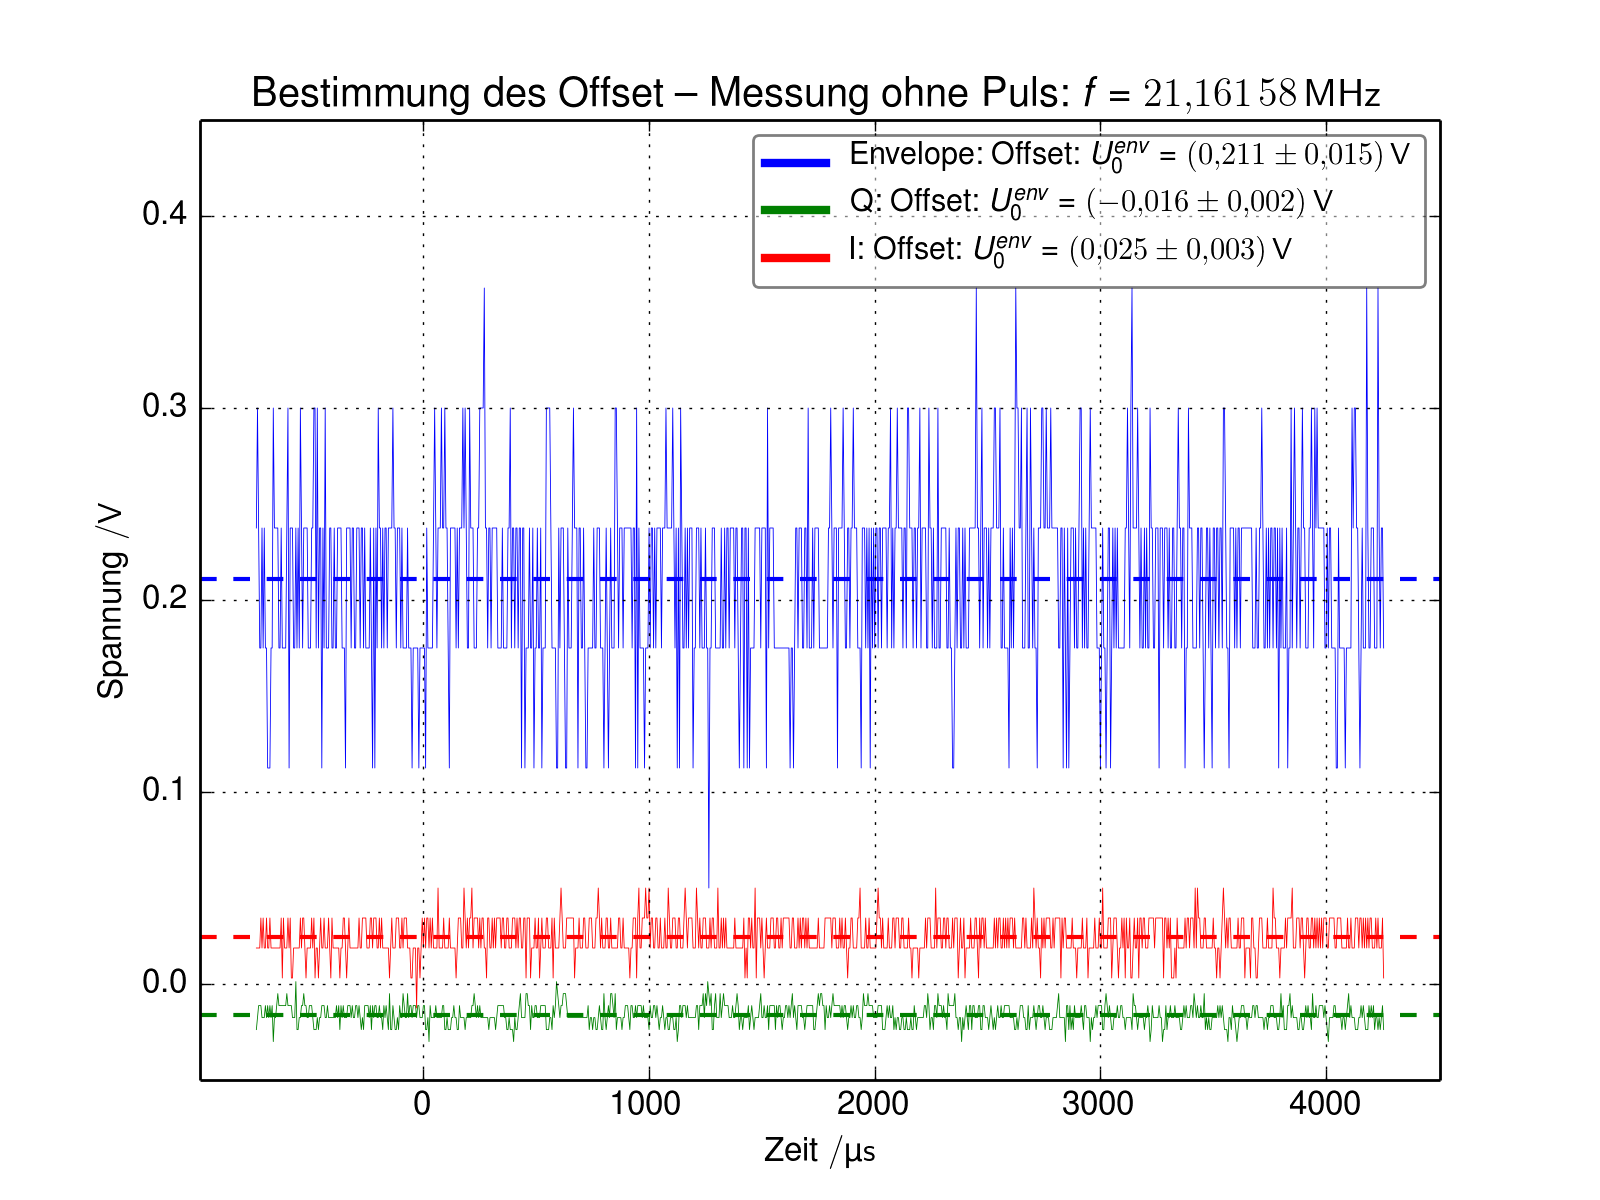
\includegraphics[width=\textwidth]{Figures/Offset.png}
        \caption{Messdaten \textbf{ohne} eingeschalteten Puls zur
          \textit{Offset} - Messung.}
        \label{AnhangfigOffset}
      \end{figure}
      
    \end{section}
    %%%%%%%%%%%%%%%%%%%%%%%%%%%%%
    
    \newpage
    %%%%%%%%%%%%%%%%%%%%%%%%%%%%%%
    %%%%%%%%%%%%%%%%%%%%%%%%%%%%%%
    %%%%%%%%%%%%%%%%%%%%%%%%%%%%%%
    \begin{section}{Free Induction Decay}
      \label{chpAnhangFID}
      \begin{figure}[htb!]
        \centering
        \begin{minipage}{.48\textwidth}
          \centering
          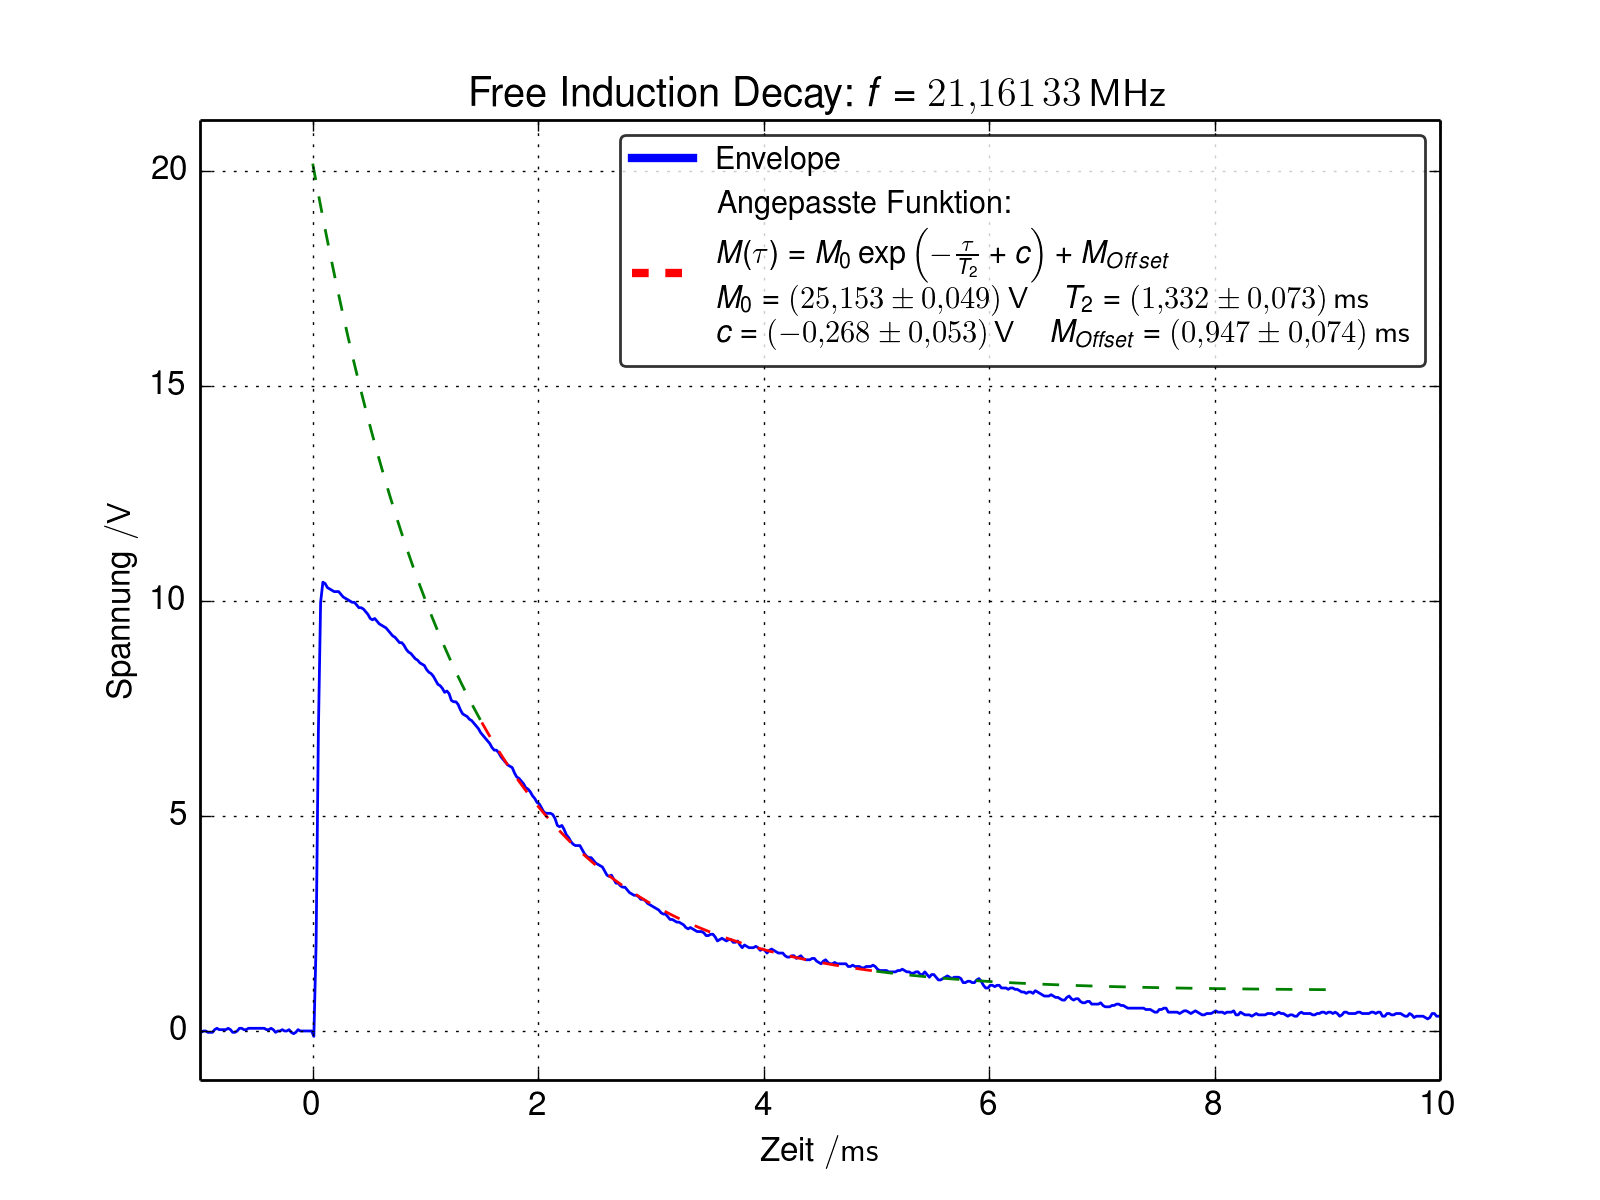
\includegraphics[width=\textwidth]{Figures/FID_env1.png}
          \caption{\textit{Free Induction Decay} Antwort - Signal und angepasste
            Zerfalls - Funktion zu beginn des Versuches.}
          \label{AnhangfigFIDenv1}
        \end{minipage}\quad
        \begin{minipage}{.48\textwidth}
          \centering
          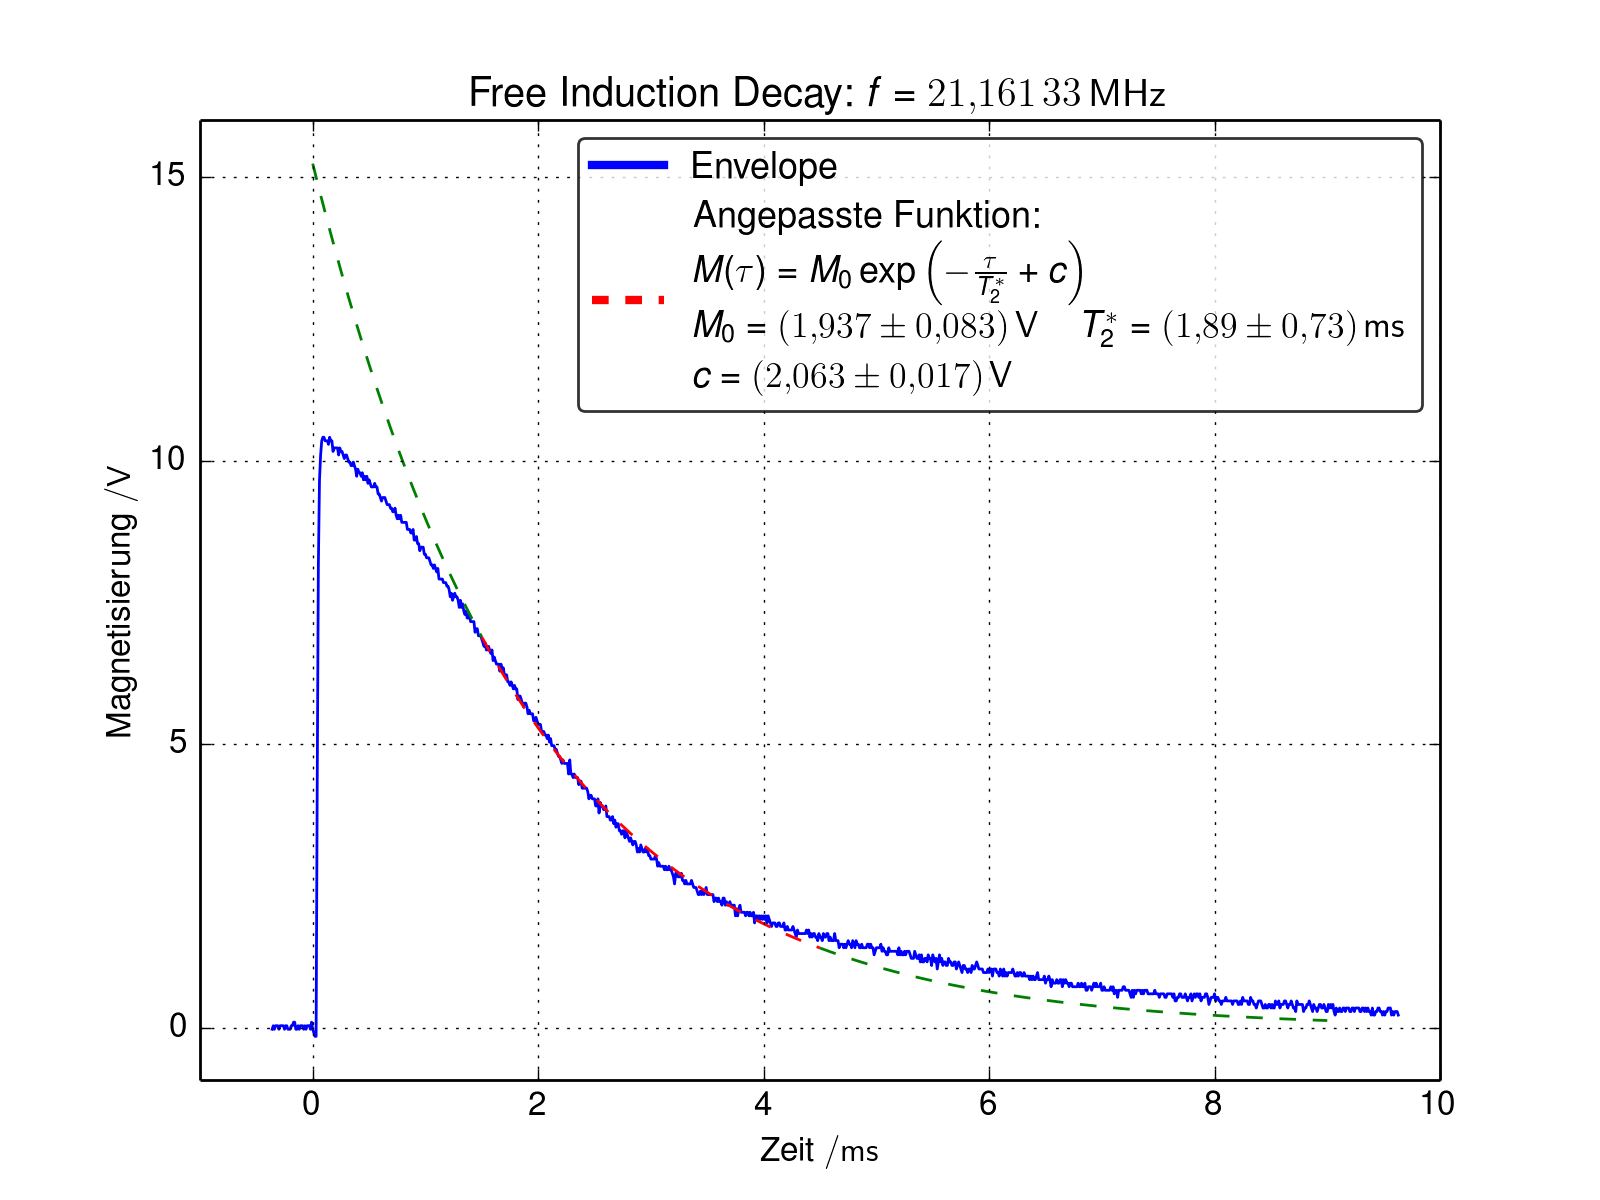
\includegraphics[width=\textwidth]{Figures/FID_env2.png}
          \caption{\textit{Free Induction Decay} Antwort - Signal und angepasste
            Zerfalls - Funktion nach der erneuten Einstellung der
            Resonanzfrequenz.}
          \label{AnhangfigFIDenv2}
        \end{minipage}\\
        \begin{minipage}{\textwidth}
          \centering
          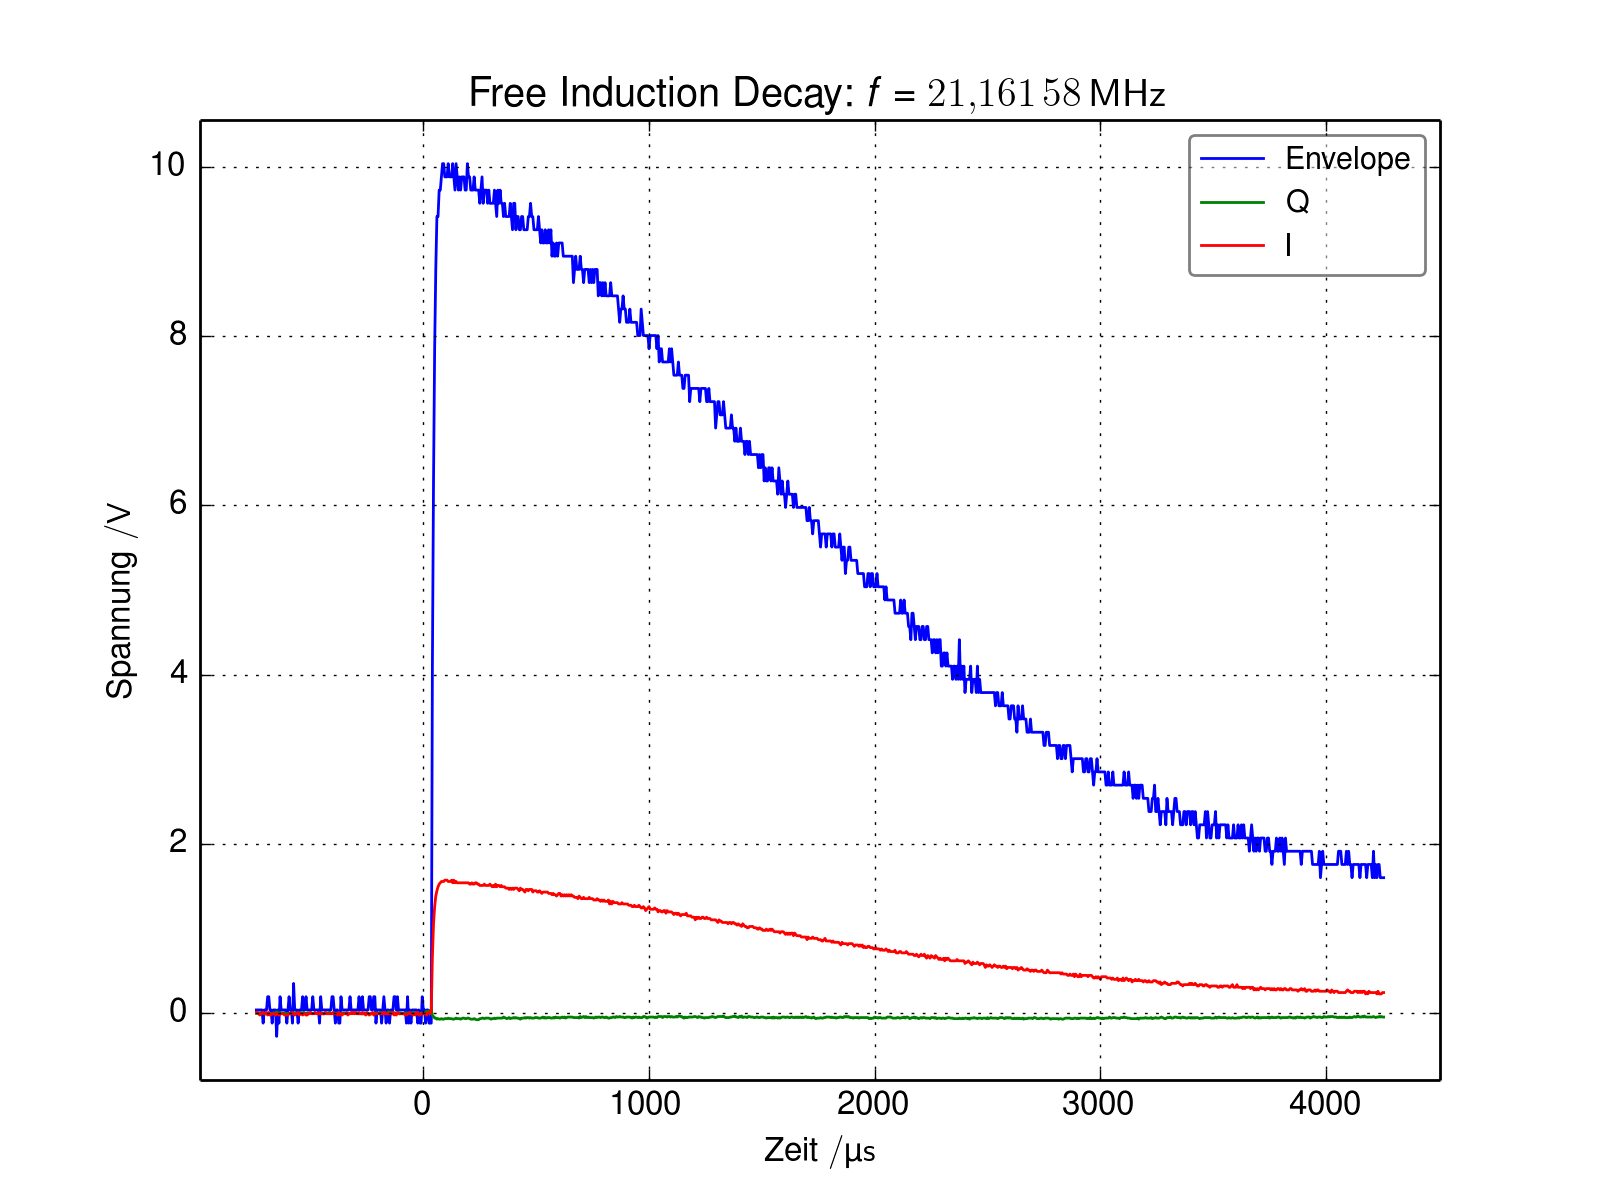
\includegraphics[width=\textwidth]{Figures/FID_env_Q_I0.png}
          \caption{\textit{Free Induction Decay} Antwort-, Q- und I - Signal.}
          \label{AnhangfigFIDenv3}
        \end{minipage}
      \end{figure}
      
    \end{section}
    %%%%%%%%%%%%%%%%%%%%%%%%%%%%%
    
    \newpage
    %%%%%%%%%%%%%%%%%%%%%%%%%%%%%%
    %%%%%%%%%%%%%%%%%%%%%%%%%%%%%%
    %%%%%%%%%%%%%%%%%%%%%%%%%%%%%%
    \begin{section}{Rabi--Oszillation}
      \label{chpAnhangRabi}
      \begin{figure}[htb]
        \centering
        \begin{minipage}{\textwidth}
          \centering
          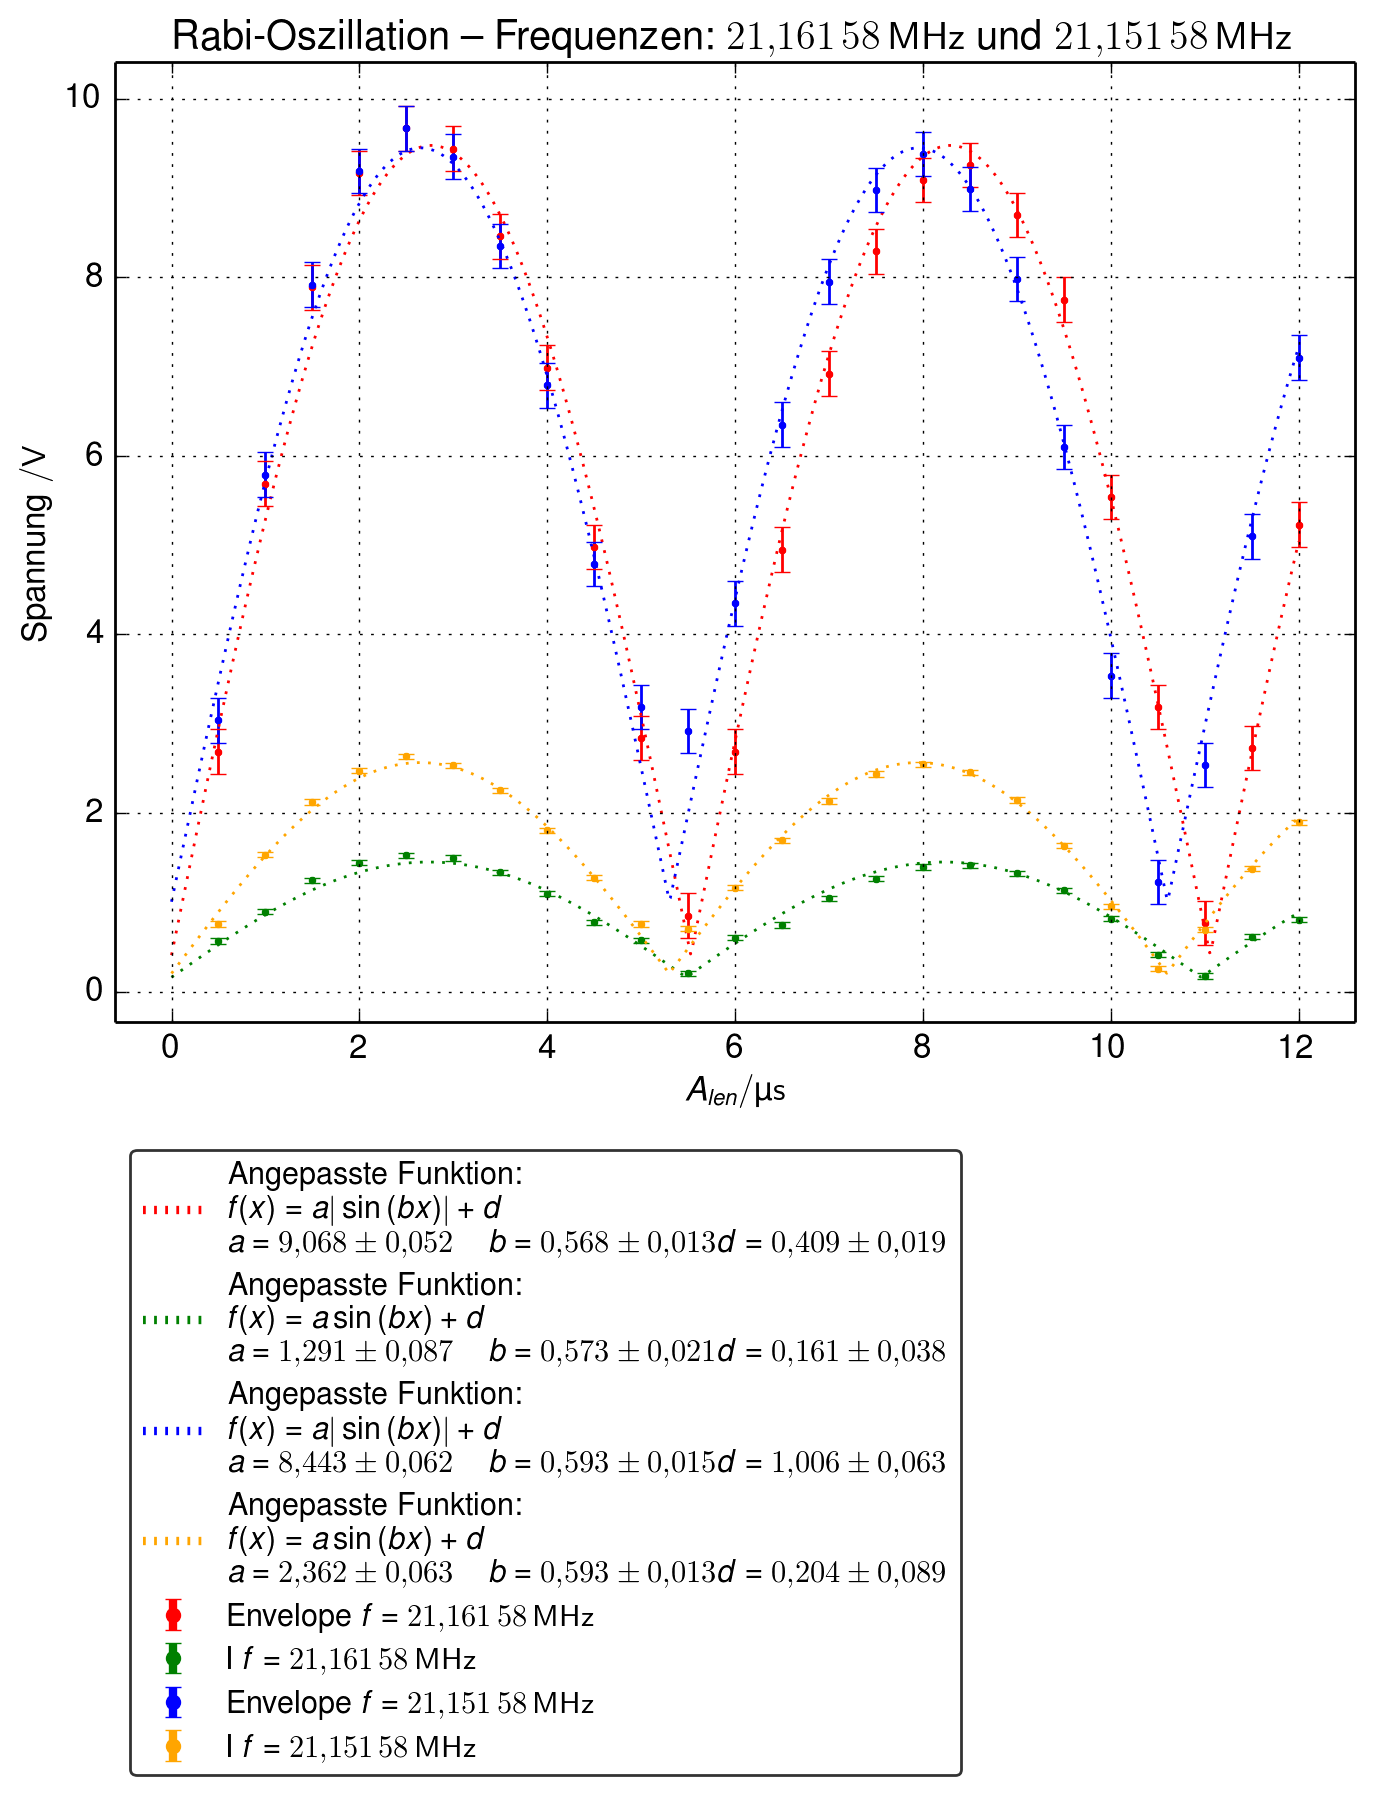
\includegraphics[width=\textwidth]{Figures/Rabi_freq12.png}
          \caption{Rabi--Oszillationen des Antwort - und In--Phase - Signales
            beider Frequenzen.}
          \label{AnhangfigRabi12}
        \end{minipage}\\
        \begin{minipage}{.48\textwidth}
          \centering
          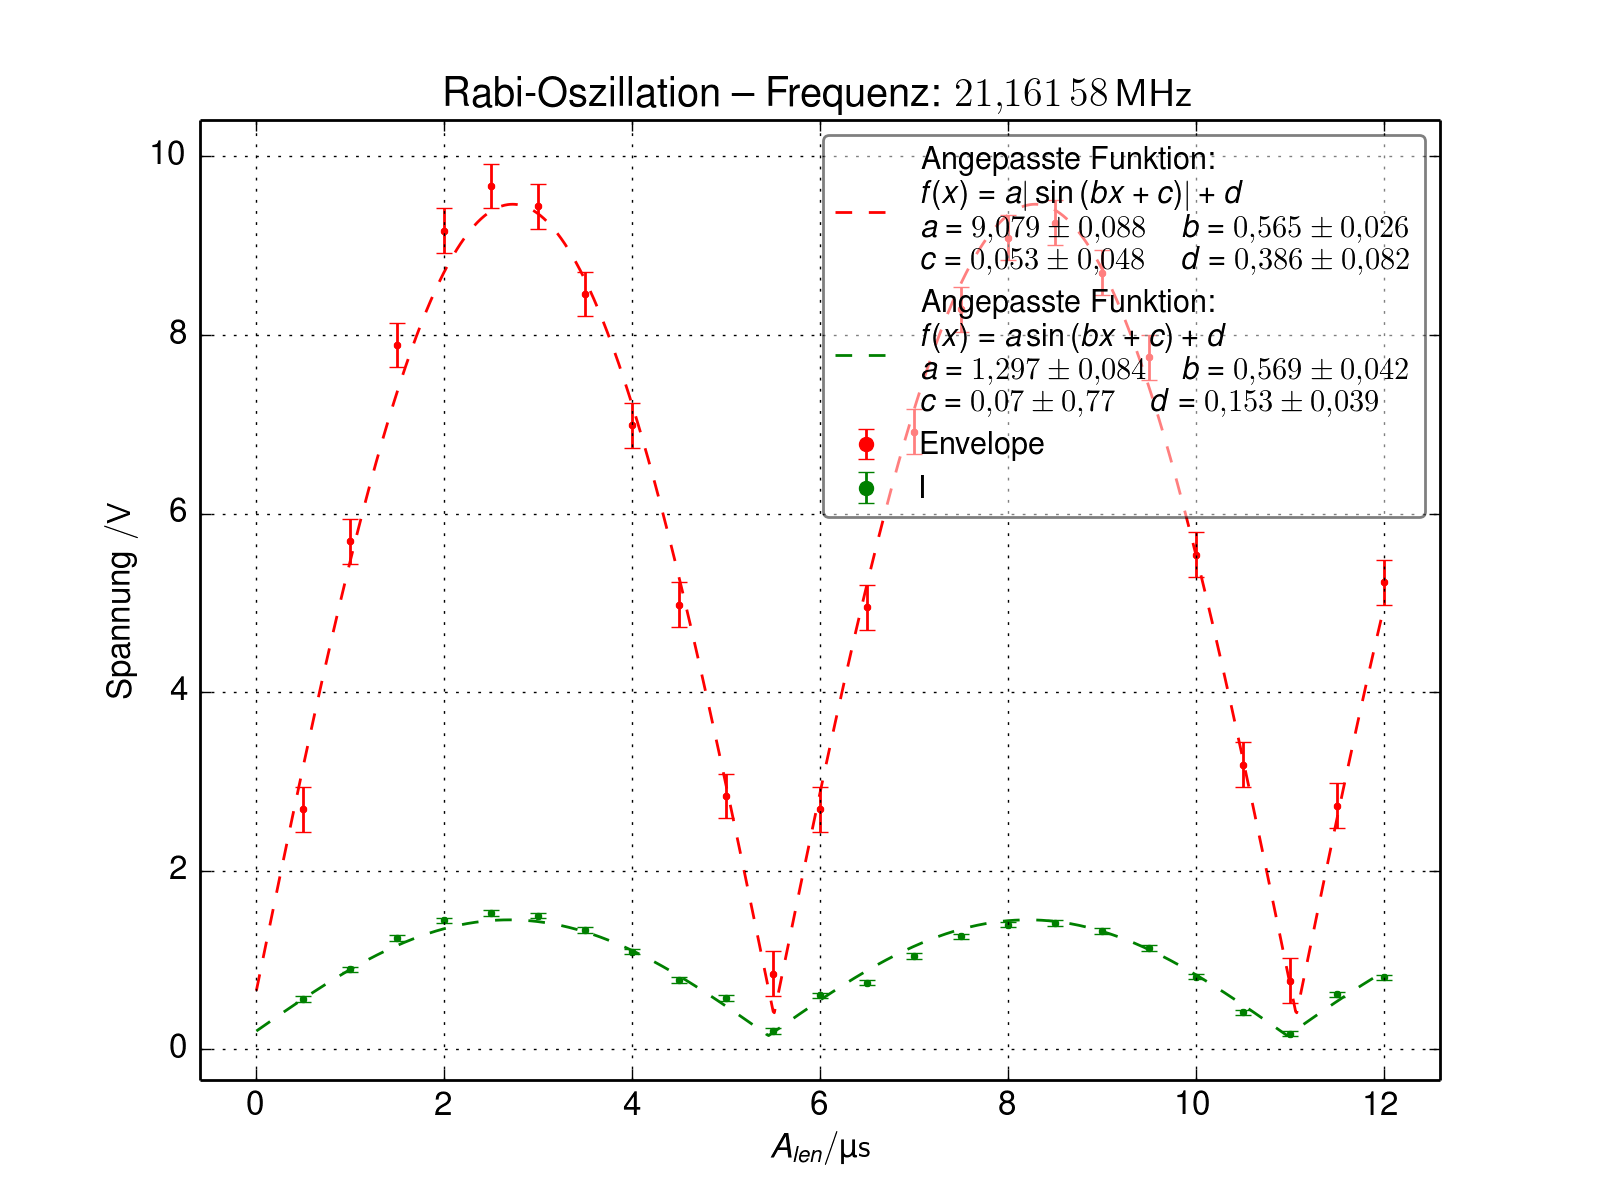
\includegraphics[width=\textwidth]{Figures/Rabi_freq1.png}
          \caption{Rabi--Oszillationen des Antwort - und In--Phase - Signales
            bei Resonanzfrequenz.}
          \label{AnhangfigRabi1}
        \end{minipage}\quad
        \begin{minipage}{.48\textwidth}
          \centering
          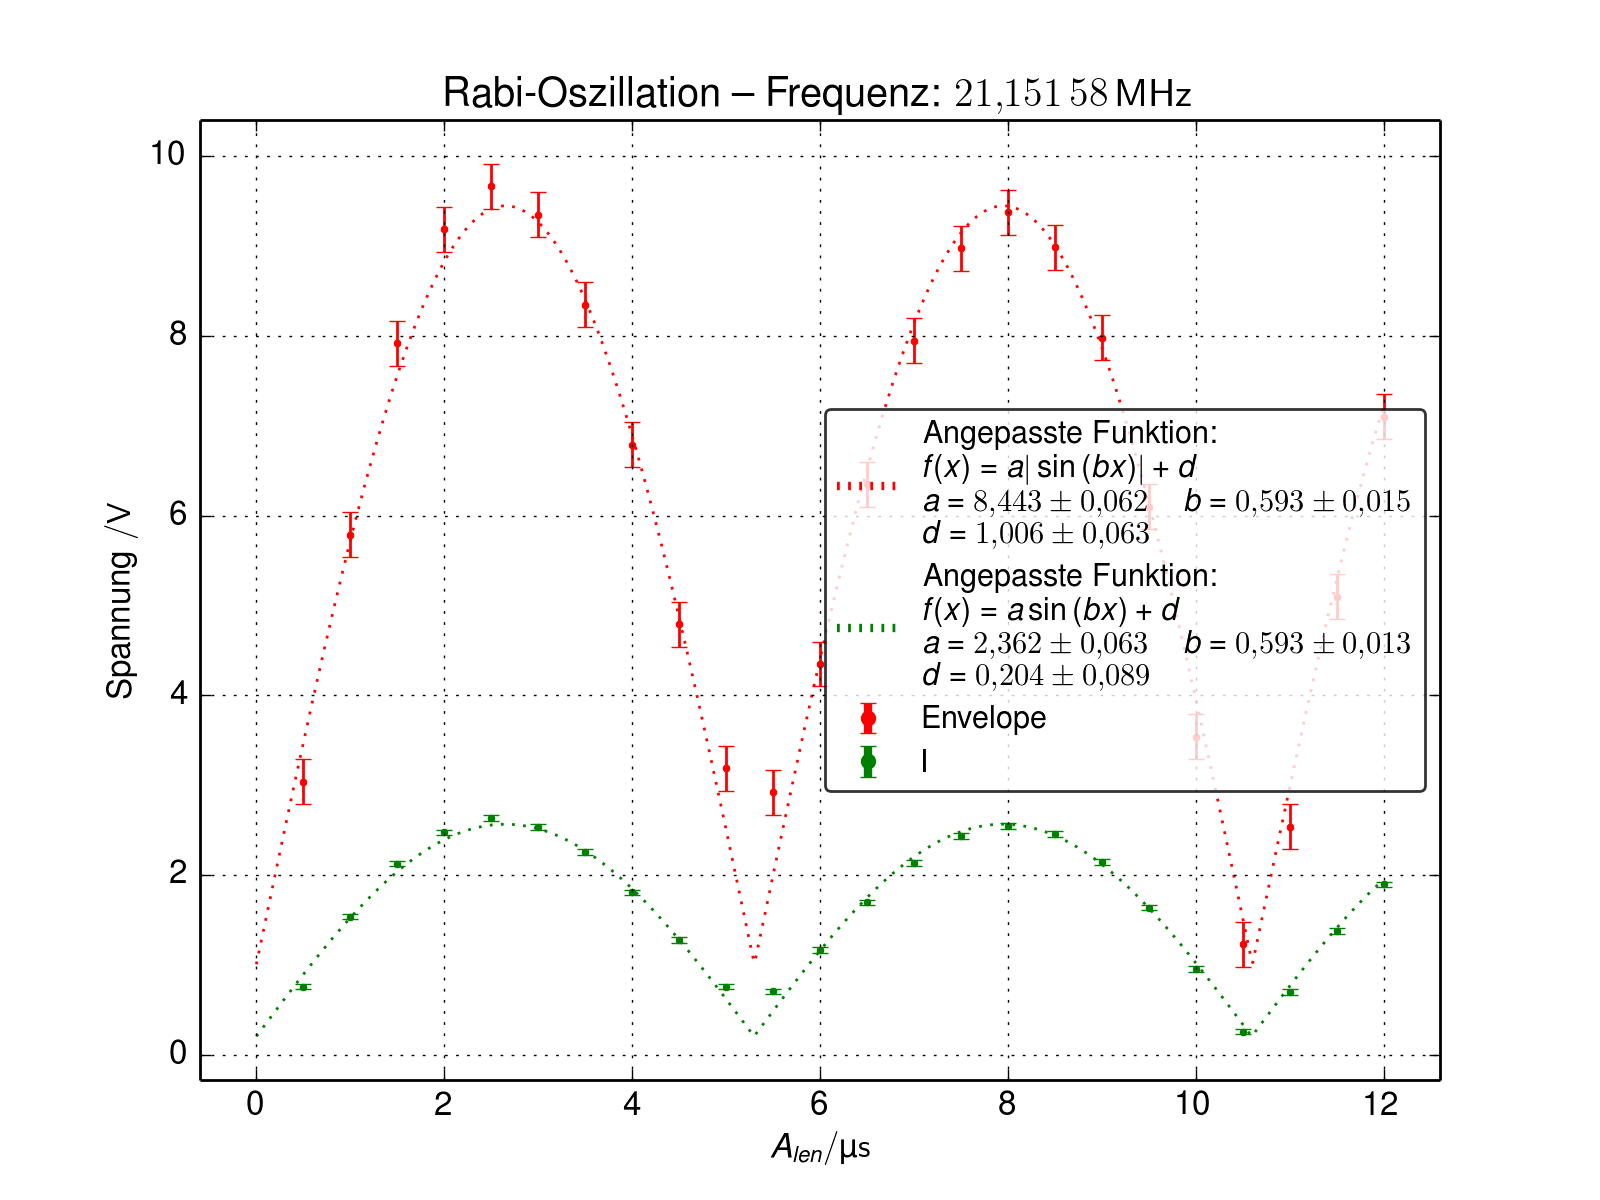
\includegraphics[width=\textwidth]{Figures/Rabi_freq2.png}
          \caption{Rabi--Oszillationen des Antwort - und In--Phase - Signales
            bei veränderter Frequenz.}
          \label{AnhangfigRabi2}
        \end{minipage}
      \end{figure}
      
    \end{section}
    %%%%%%%%%%%%%%%%%%%%%%%%%%%%%
    
    \newpage
    %%%%%%%%%%%%%%%%%%%%%%%%%%%%%%
    %%%%%%%%%%%%%%%%%%%%%%%%%%%%%%
    %%%%%%%%%%%%%%%%%%%%%%%%%%%%%%
    \begin{section}{Longitudinale Relaxationszeit}
      \label{chpAnhangLong}
      \begin{figure}[htb!]
        \centering
        \begin{minipage}{\textwidth}
          \centering
          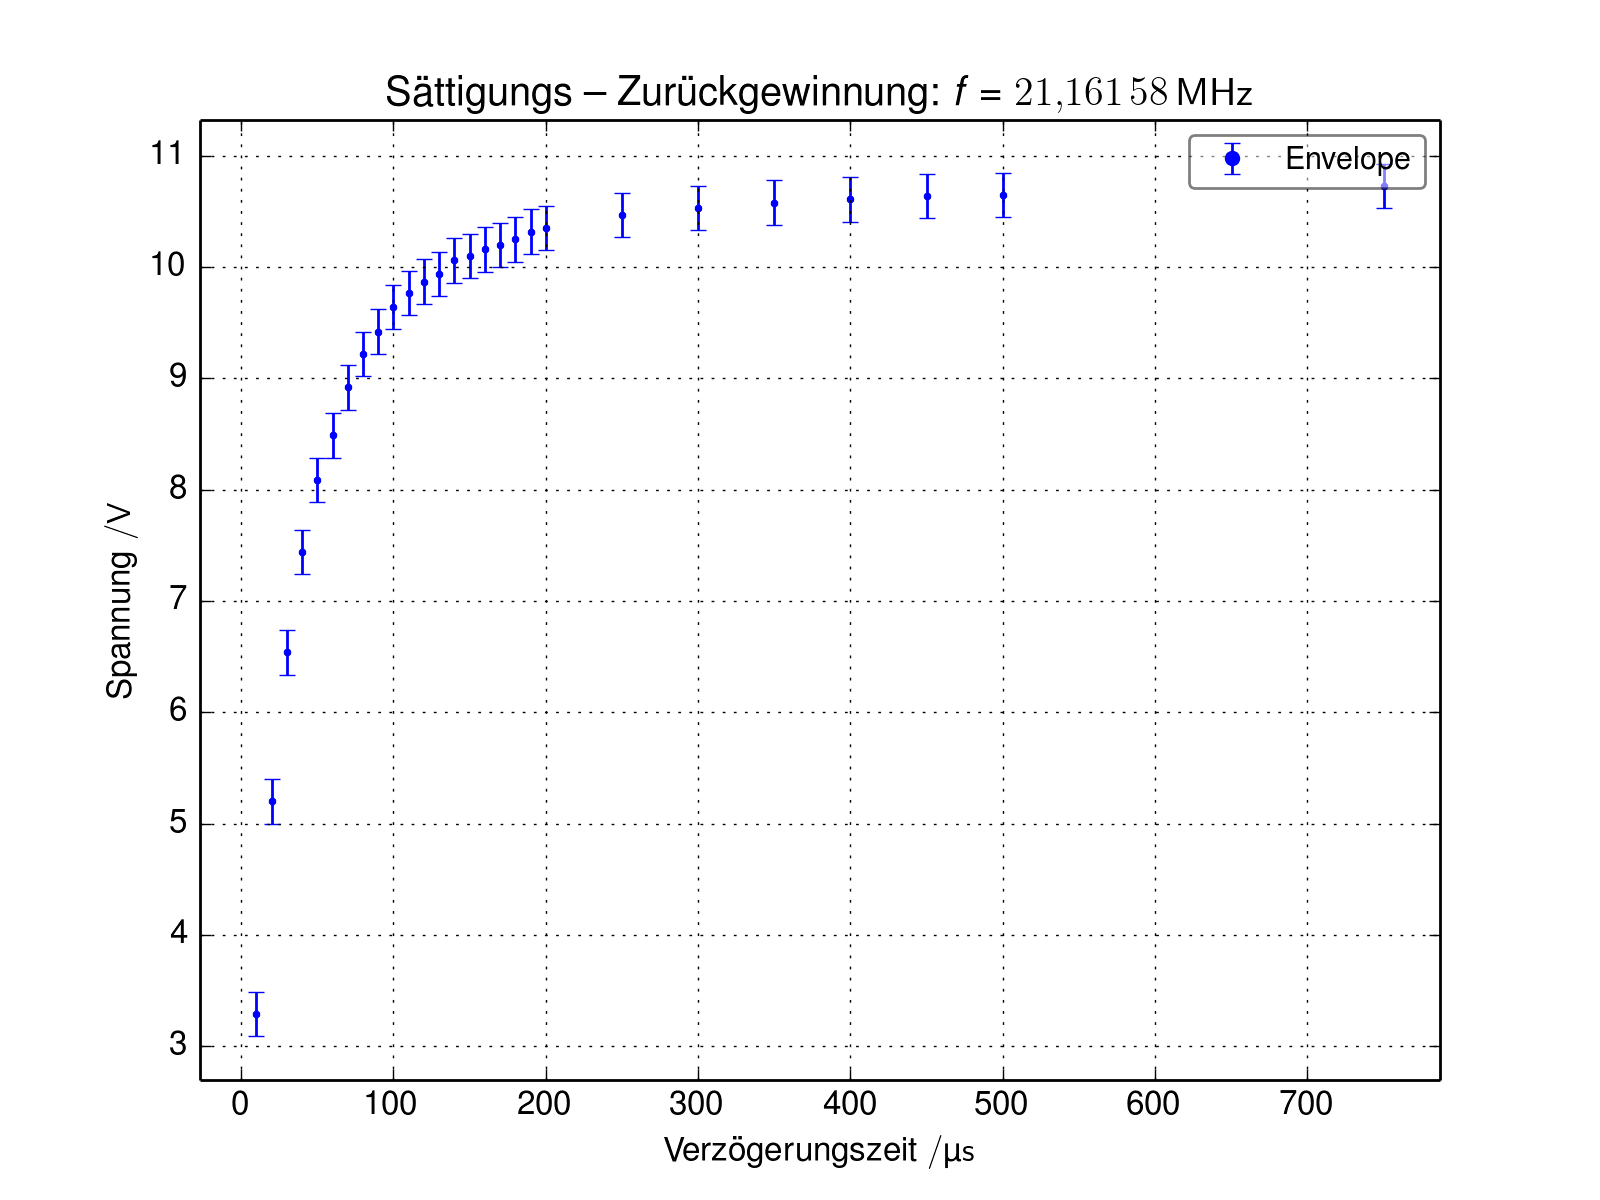
\includegraphics[width=\textwidth]
          {Figures/SaettigungsZurueckgewinnung.png}
          \caption{Verlauf der maximalen Spannung des Antwort - Signales bei
            der Sättigungs--Zurückgewinnungs - Methode.}
          \label{AnhangfigSaettigung}
        \end{minipage}\\
        \begin{minipage}{\textwidth}
          \centering
          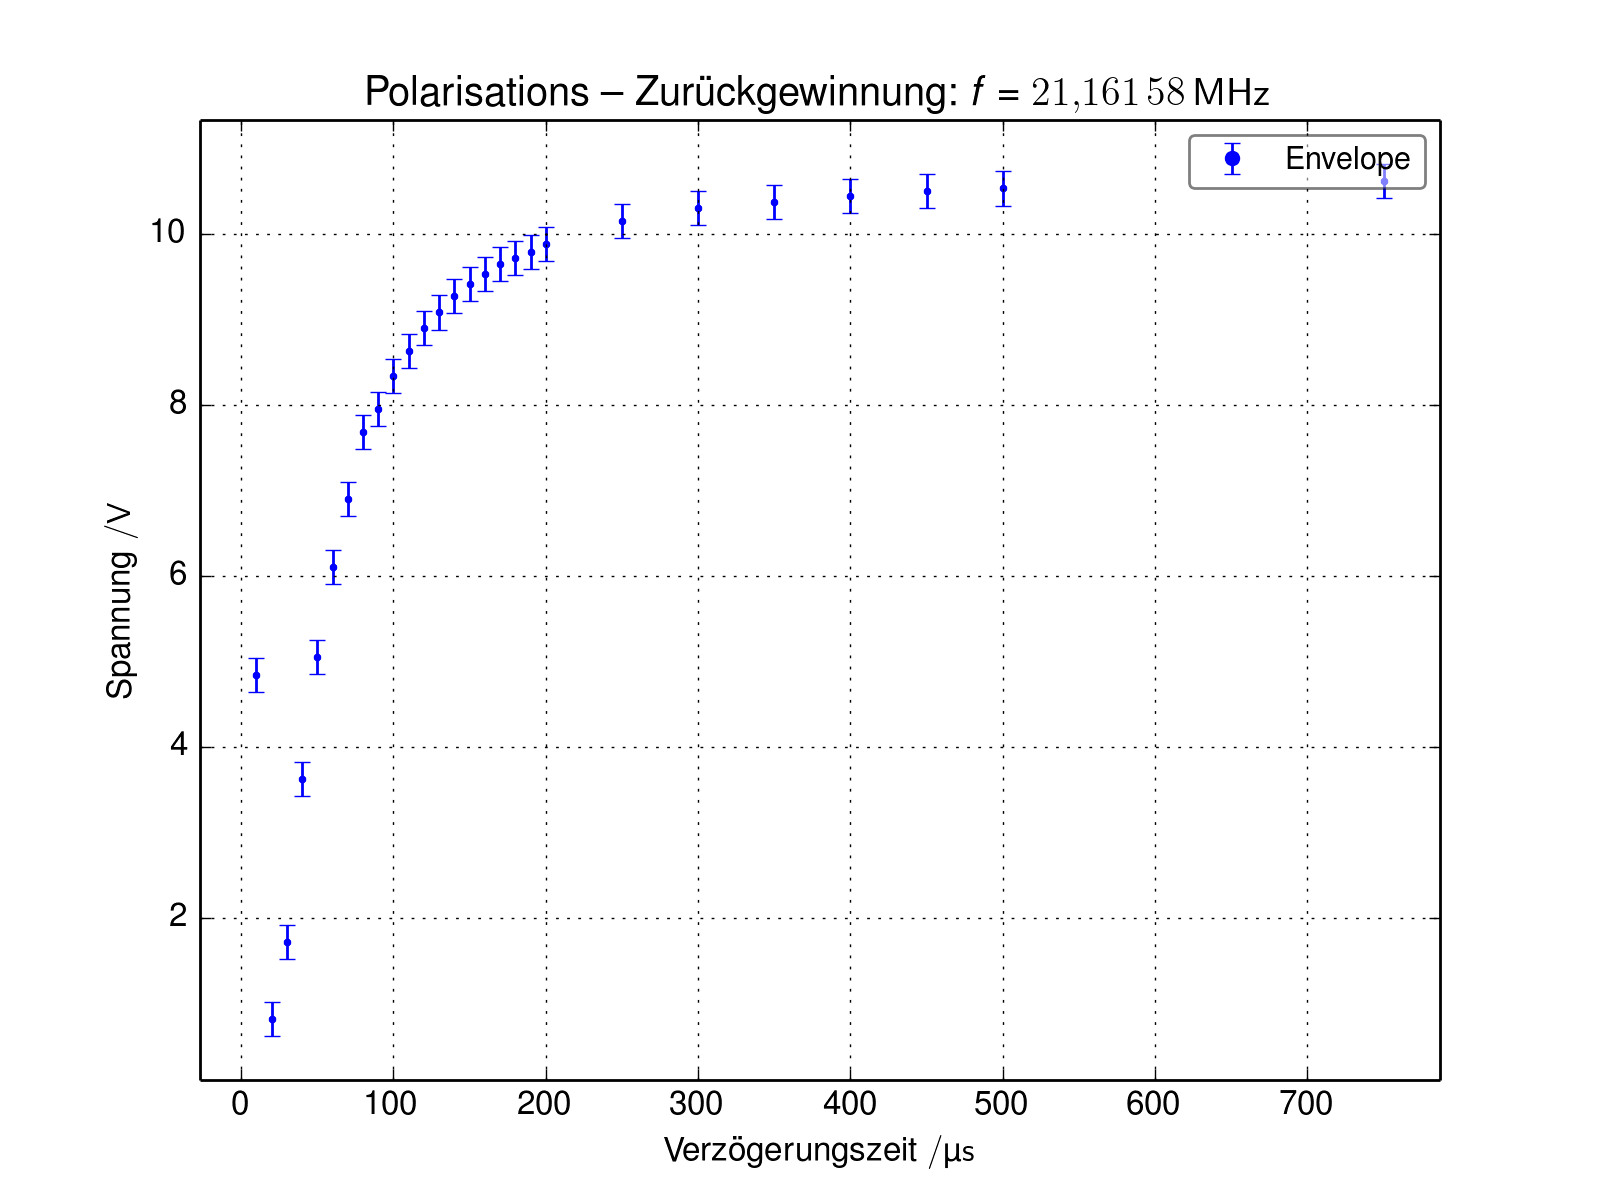
\includegraphics[width=\textwidth]
          {Figures/PolarisationsZurueckgewinnung.png}
          \caption{Verlauf der maximalen Spannung des Antwort - Signales bei
            der Polarisations--Zurückgewinnungs - Methode.}
          \label{AnhangfigPolarisation}
        \end{minipage}
      \end{figure}
      
    \end{section}
    %%%%%%%%%%%%%%%%%%%%%%%%%%%%%
    
    \newpage
    %%%%%%%%%%%%%%%%%%%%%%%%%%%%%%
    %%%%%%%%%%%%%%%%%%%%%%%%%%%%%%
    %%%%%%%%%%%%%%%%%%%%%%%%%%%%%%
    \begin{section}{Homogene Transversale Relaxationszeit}
      \label{chpAnhangTrans}
      
      %%%%%%%%%%%%%%%%%%%%%%%%%%%%%%%%%%%%%%%
      %%%%%%%%%%%%%%%%%%%%%%%%%%%%%%%%%%%%%%%
      %%%%%%%%%%%%%%%%%%%%%%%%%%%%%%%%%%%%%%%
      \begin{subsection}*{Hahn--Spinecho - Sequenz}
        \label{chpAnhangTransHahn}
        \begin{figure}[htb]
          \centering
          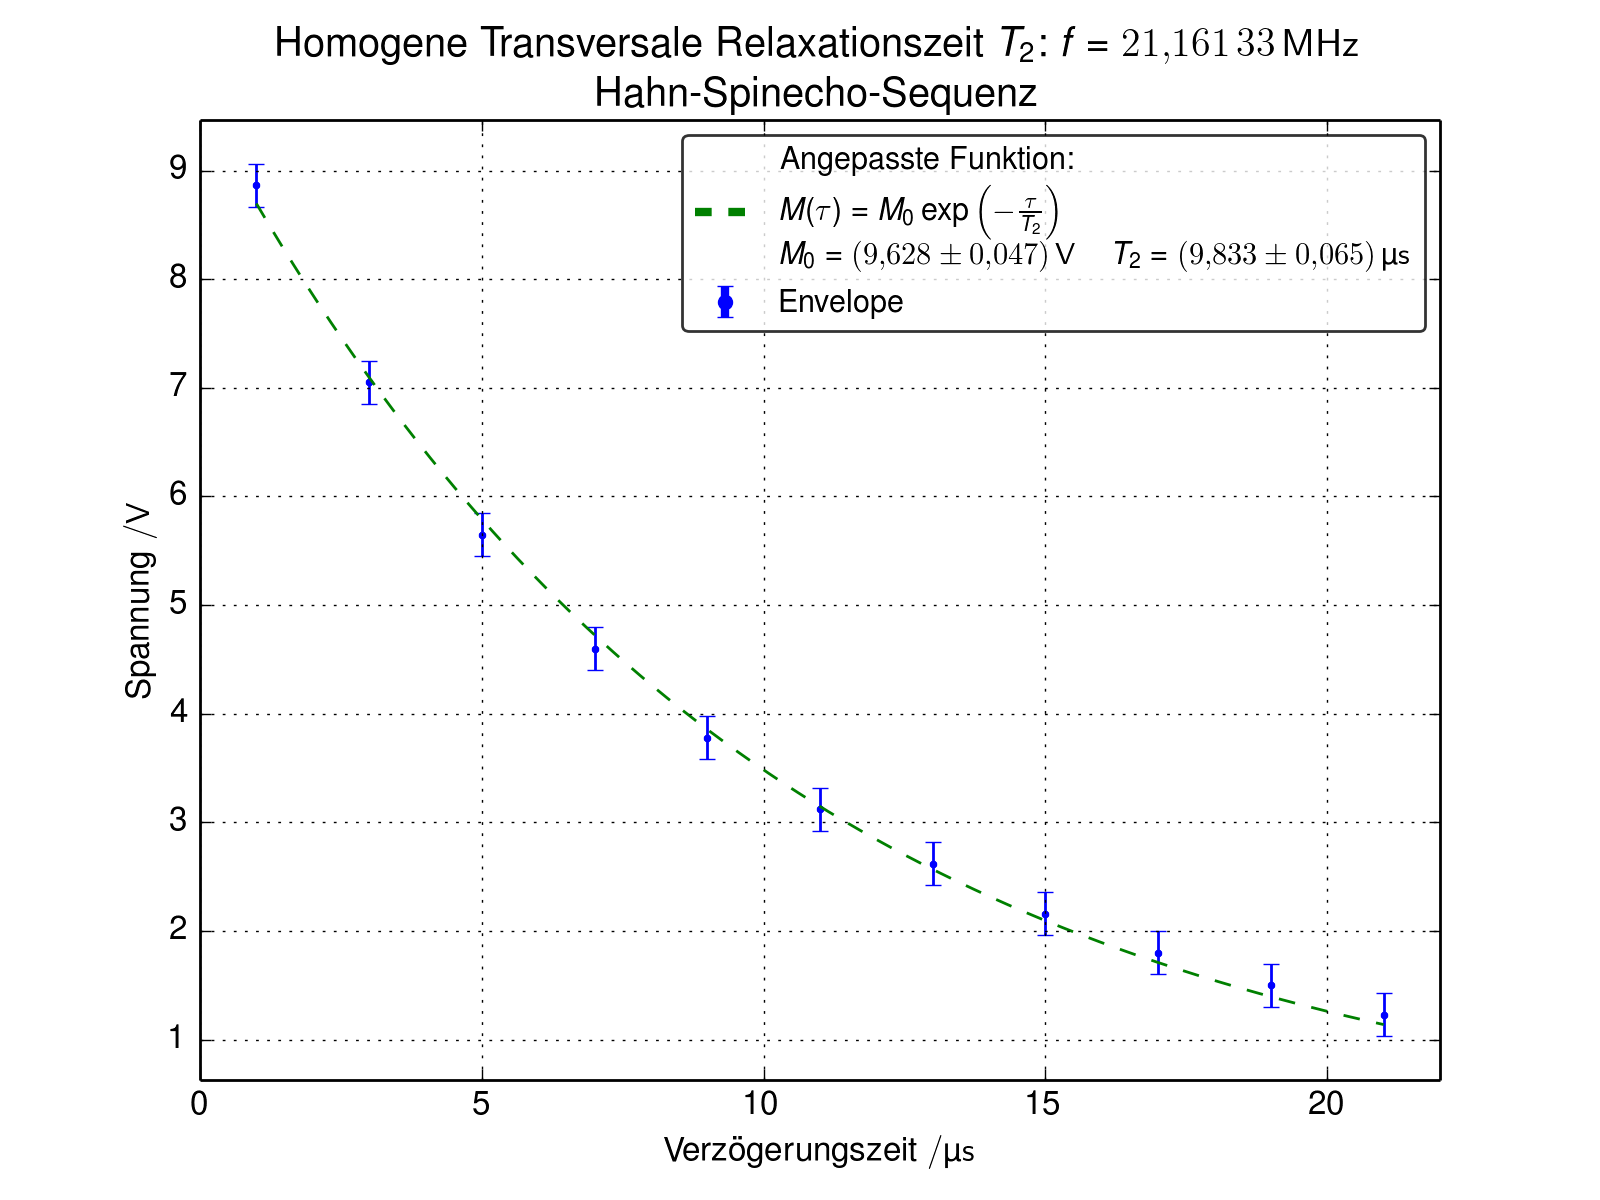
\includegraphics[width=\textwidth]
          {Figures/HomoTransRelax_Hahn.png}
          \caption{Verlauf der maximalen Spannung des Echo - Signales bei der
            Hahn--Spinecho - Sequenz.}
          \label{AnhangfigHahn}
        \end{figure}
        \begin{figure}[htb]
          \centering
          \begin{minipage}{.48\textwidth}
            \centering
            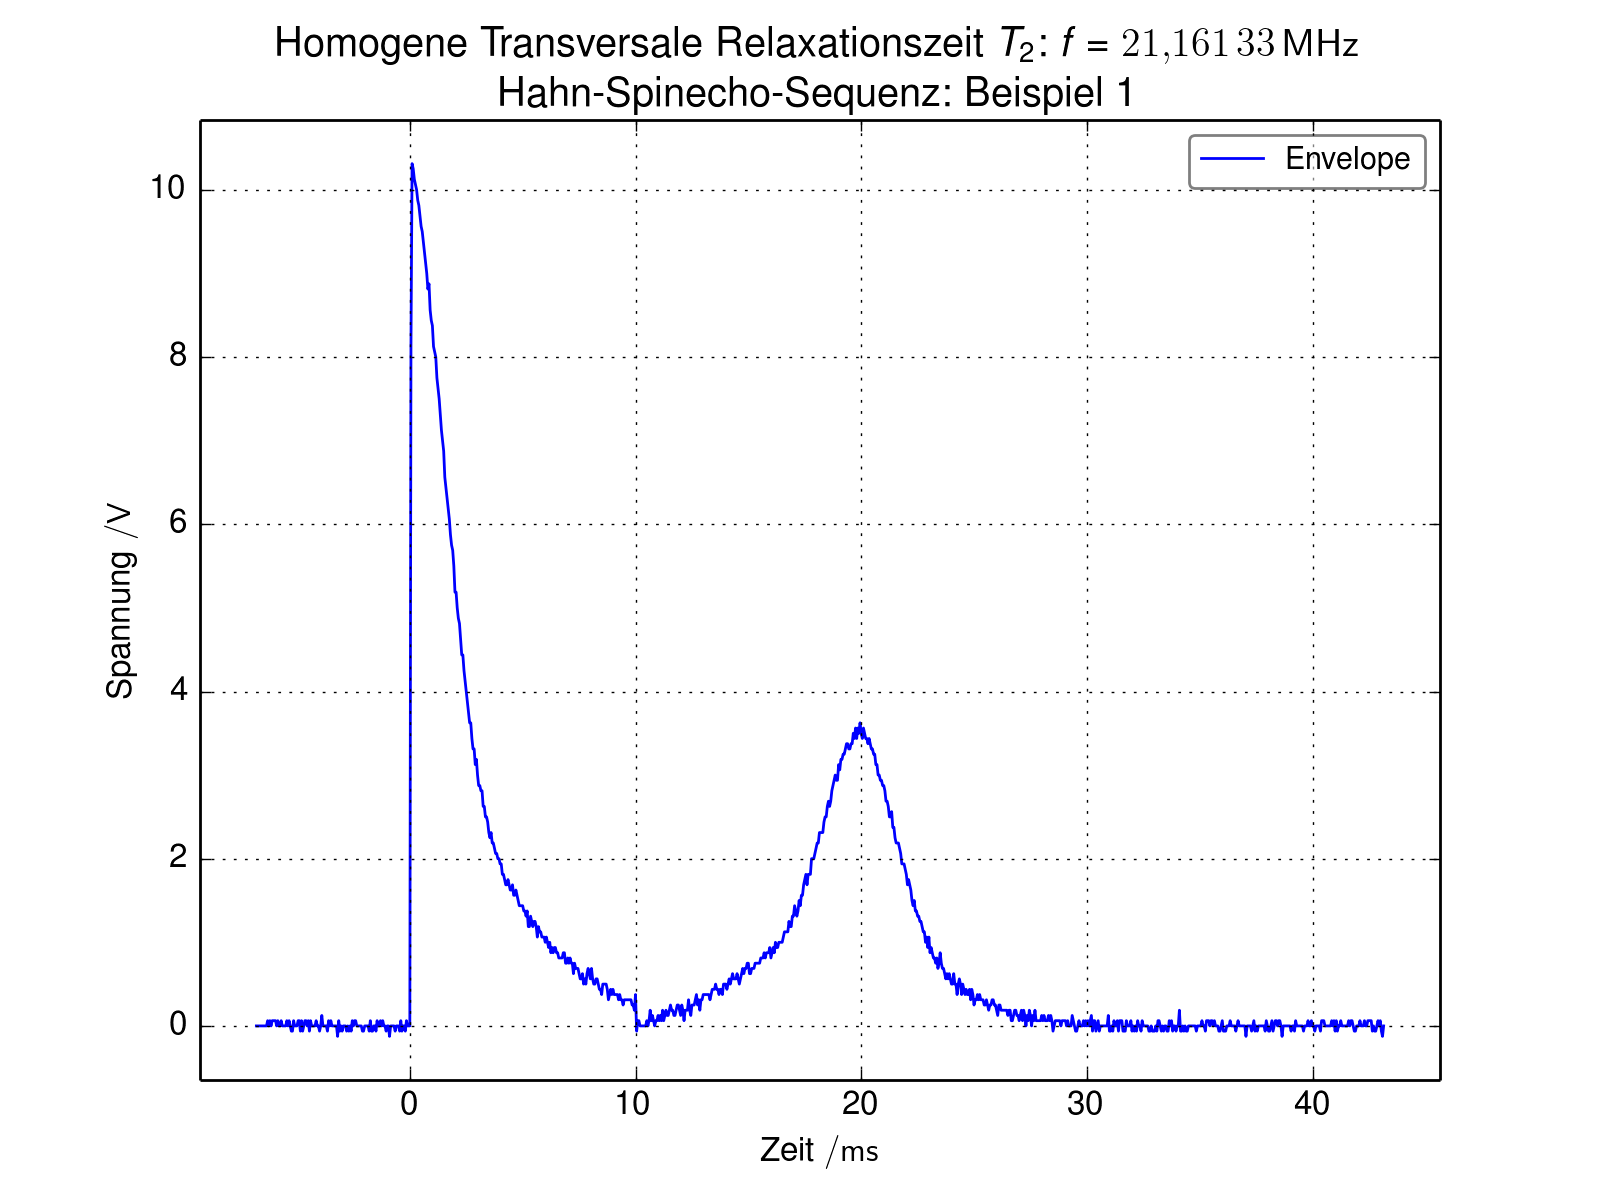
\includegraphics[width=\textwidth]
            {Figures/HomoTransRelax_Hahn_beispiel0.png}
            \caption{Beispiel eines Antwort - Signales bei der
              Hahn--Spinecho - Sequenz.}
            \label{AnhangfigHahnBsp1}
          \end{minipage}\quad
          \begin{minipage}{.48\textwidth}
            \centering
            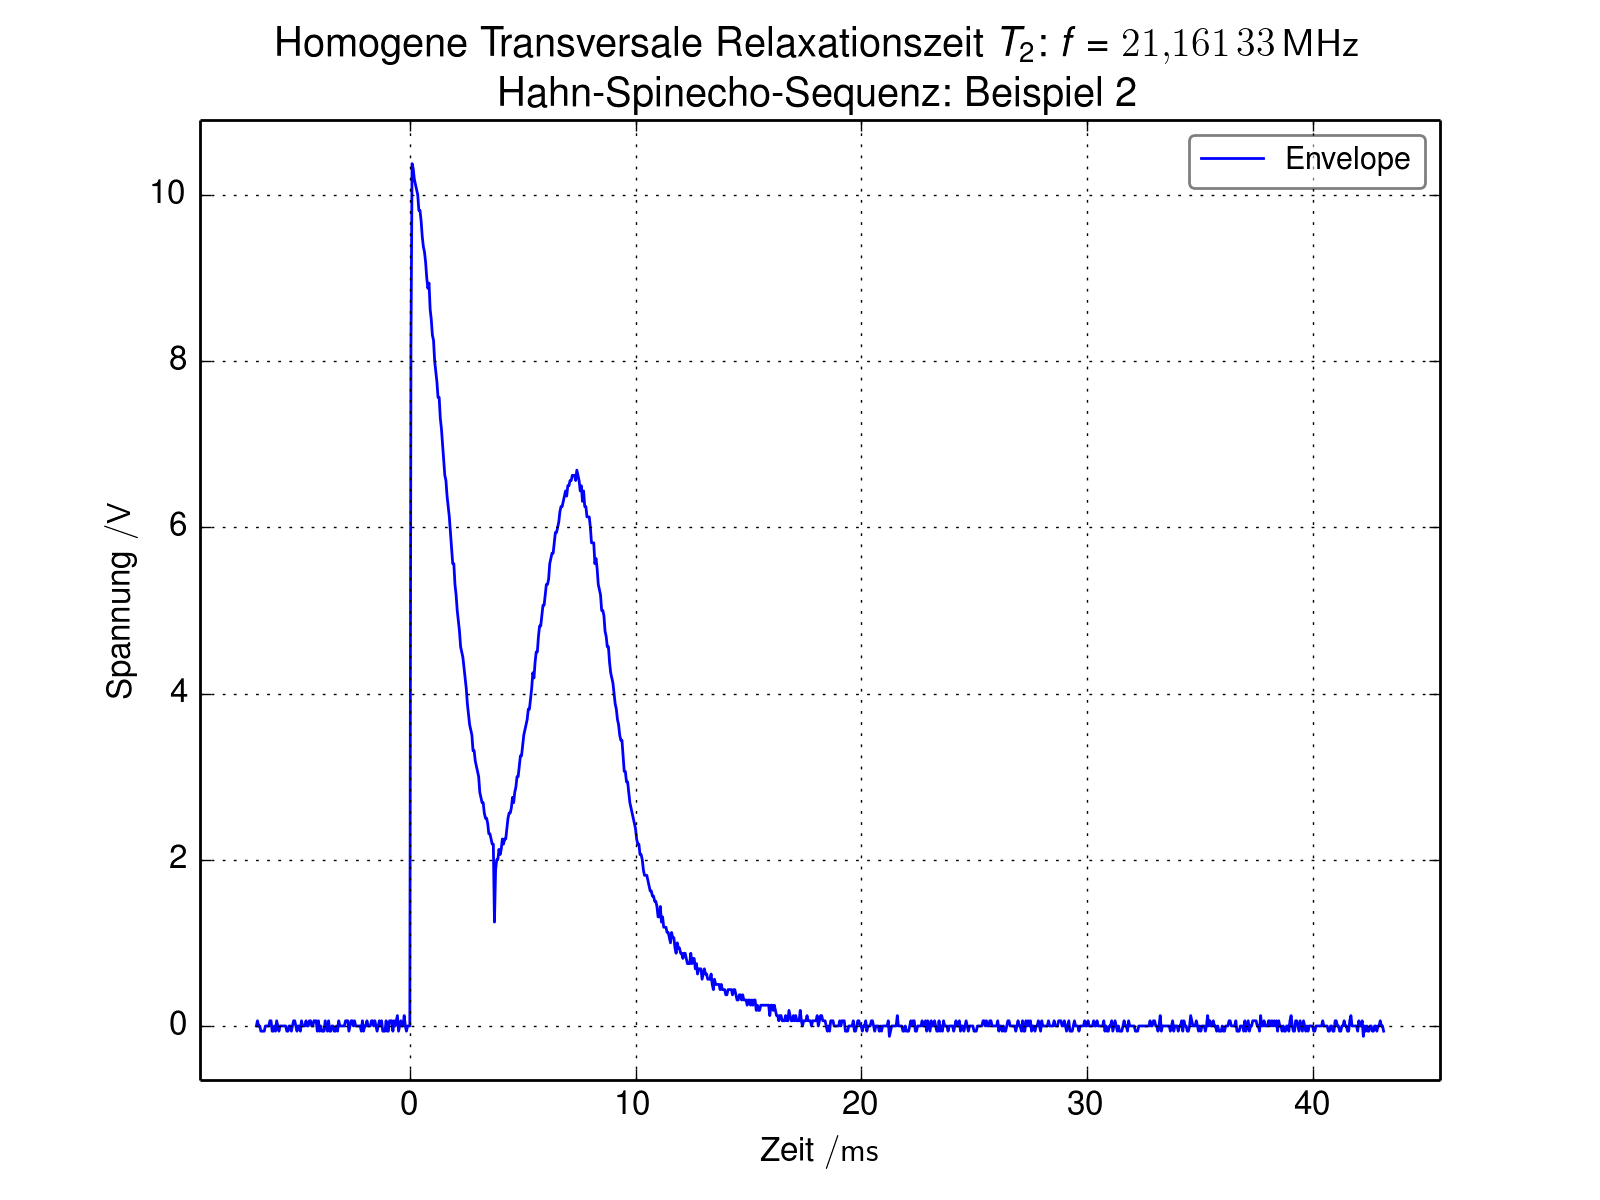
\includegraphics[width=\textwidth]
            {Figures/HomoTransRelax_Hahn_beispiel1.png}
            \caption{Beispiel eines Antwort - Signales bei der
              Hahn--Spinecho - Sequenz.}
            \label{AnhangfigHahnBsp2}
          \end{minipage}
        \end{figure}
        
      \end{subsection}
      %%%%%%%%%%%%%%%%%%%%%%%%%%%%%%%%%%%%%%%
      
      \newpage
      %%%%%%%%%%%%%%%%%%%%%%%%%%%%%%%%%%%%%%%
      %%%%%%%%%%%%%%%%%%%%%%%%%%%%%%%%%%%%%%%
      %%%%%%%%%%%%%%%%%%%%%%%%%%%%%%%%%%%%%%%
      \begin{subsection}*{Carr--Purcell - Sequenz}
        \label{chpAnhangTransCarr}
        \begin{figure}[htb!]
          \centering
          \begin{minipage}{.48\textwidth}
            \centering
            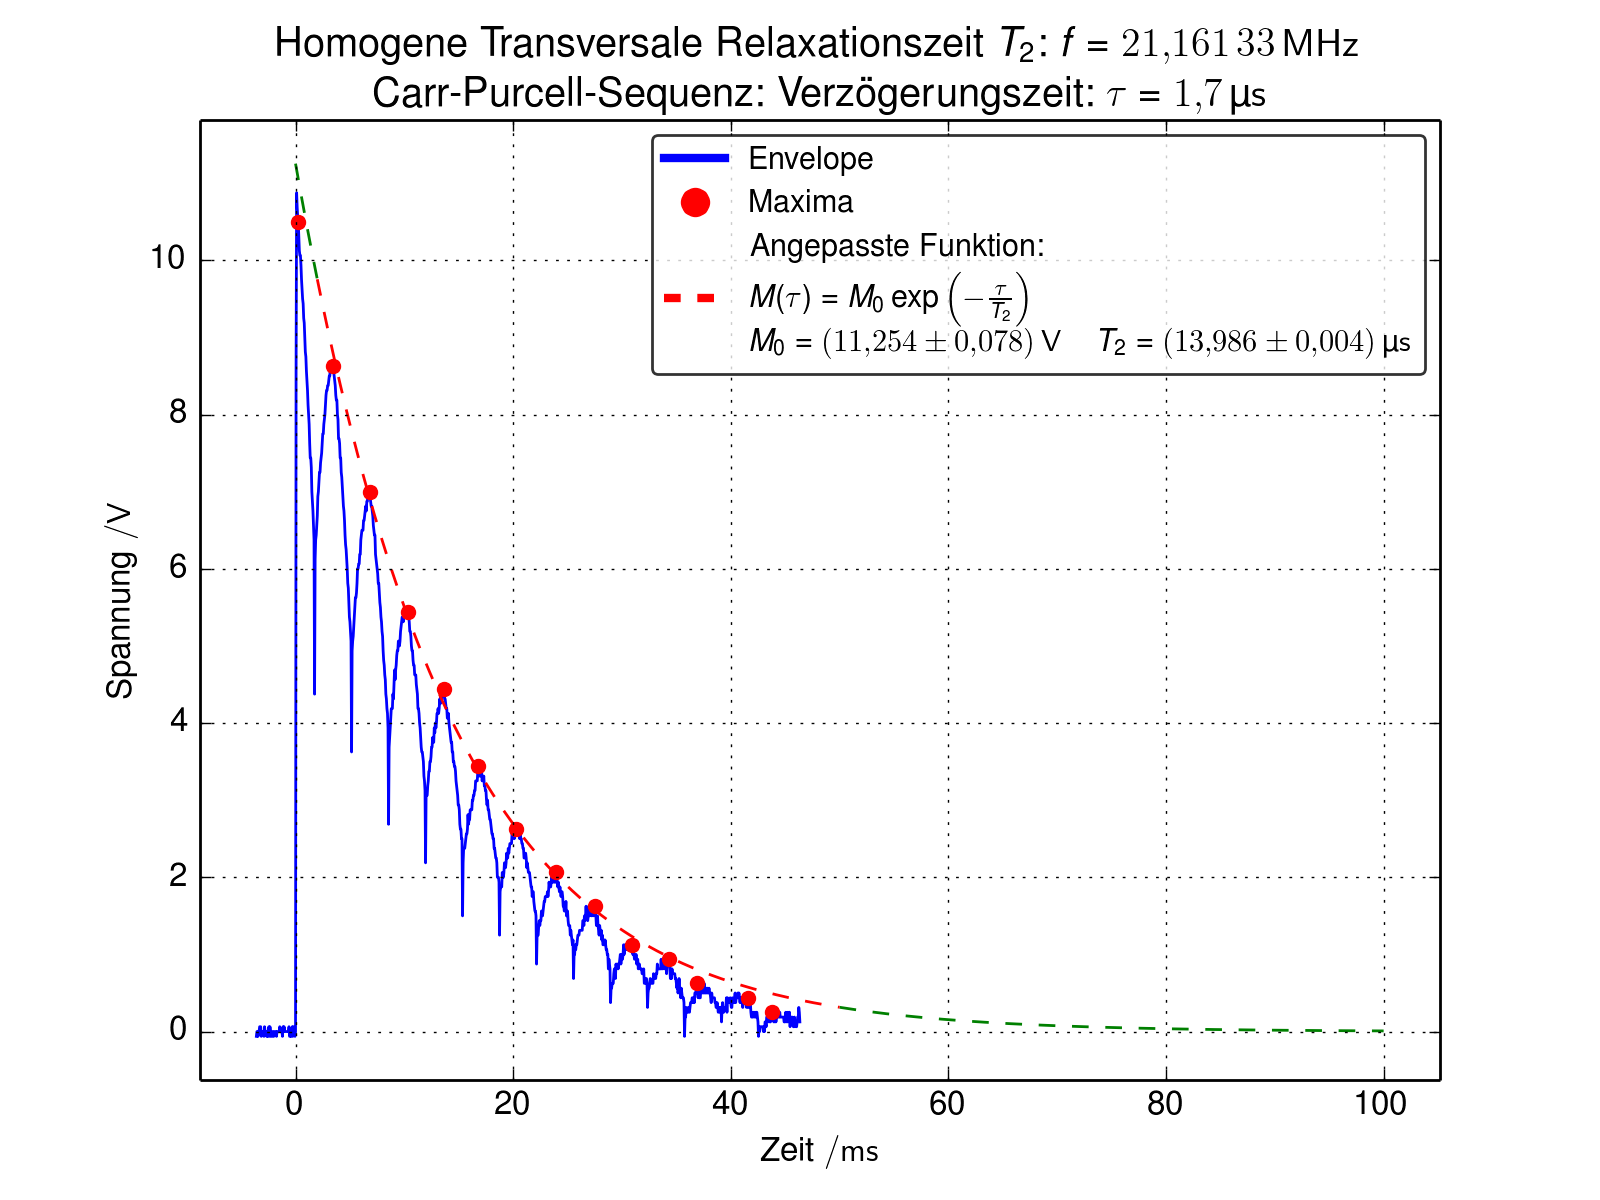
\includegraphics[width=\textwidth]
            {Figures/HomoTransRelax_Carr0.png}
            \caption{Verzögerungszeit von
              $\tau = \SI{1.7}{\micro\second}$.}
            \label{AnhangfigCarr0}
          \end{minipage}\quad
          \begin{minipage}{.48\textwidth}
            \centering
            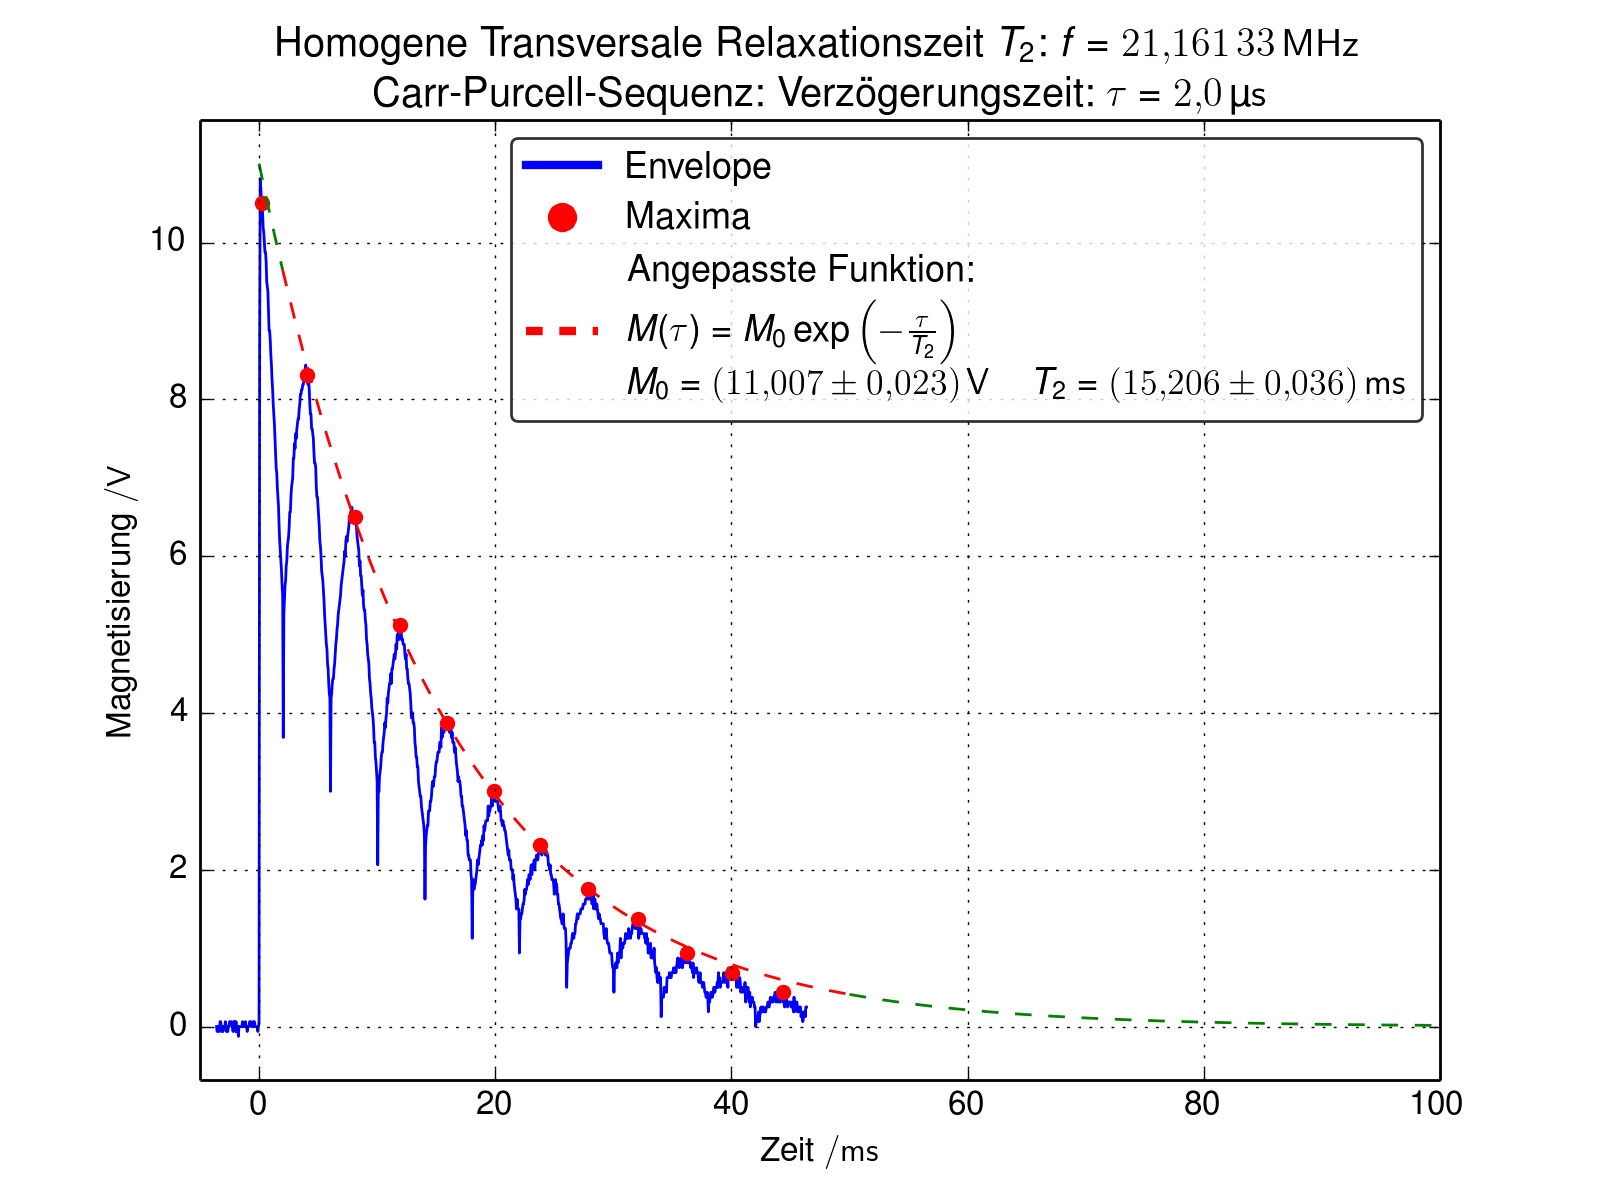
\includegraphics[width=\textwidth]
            {Figures/HomoTransRelax_Carr1.png}
            \caption{Verzögerungszeit von
              $\tau = \SI{2.0}{\micro\second}$.}
            \label{AnhangfigCarr1}
          \end{minipage}\\
          \begin{minipage}{.48\textwidth}
            \centering
            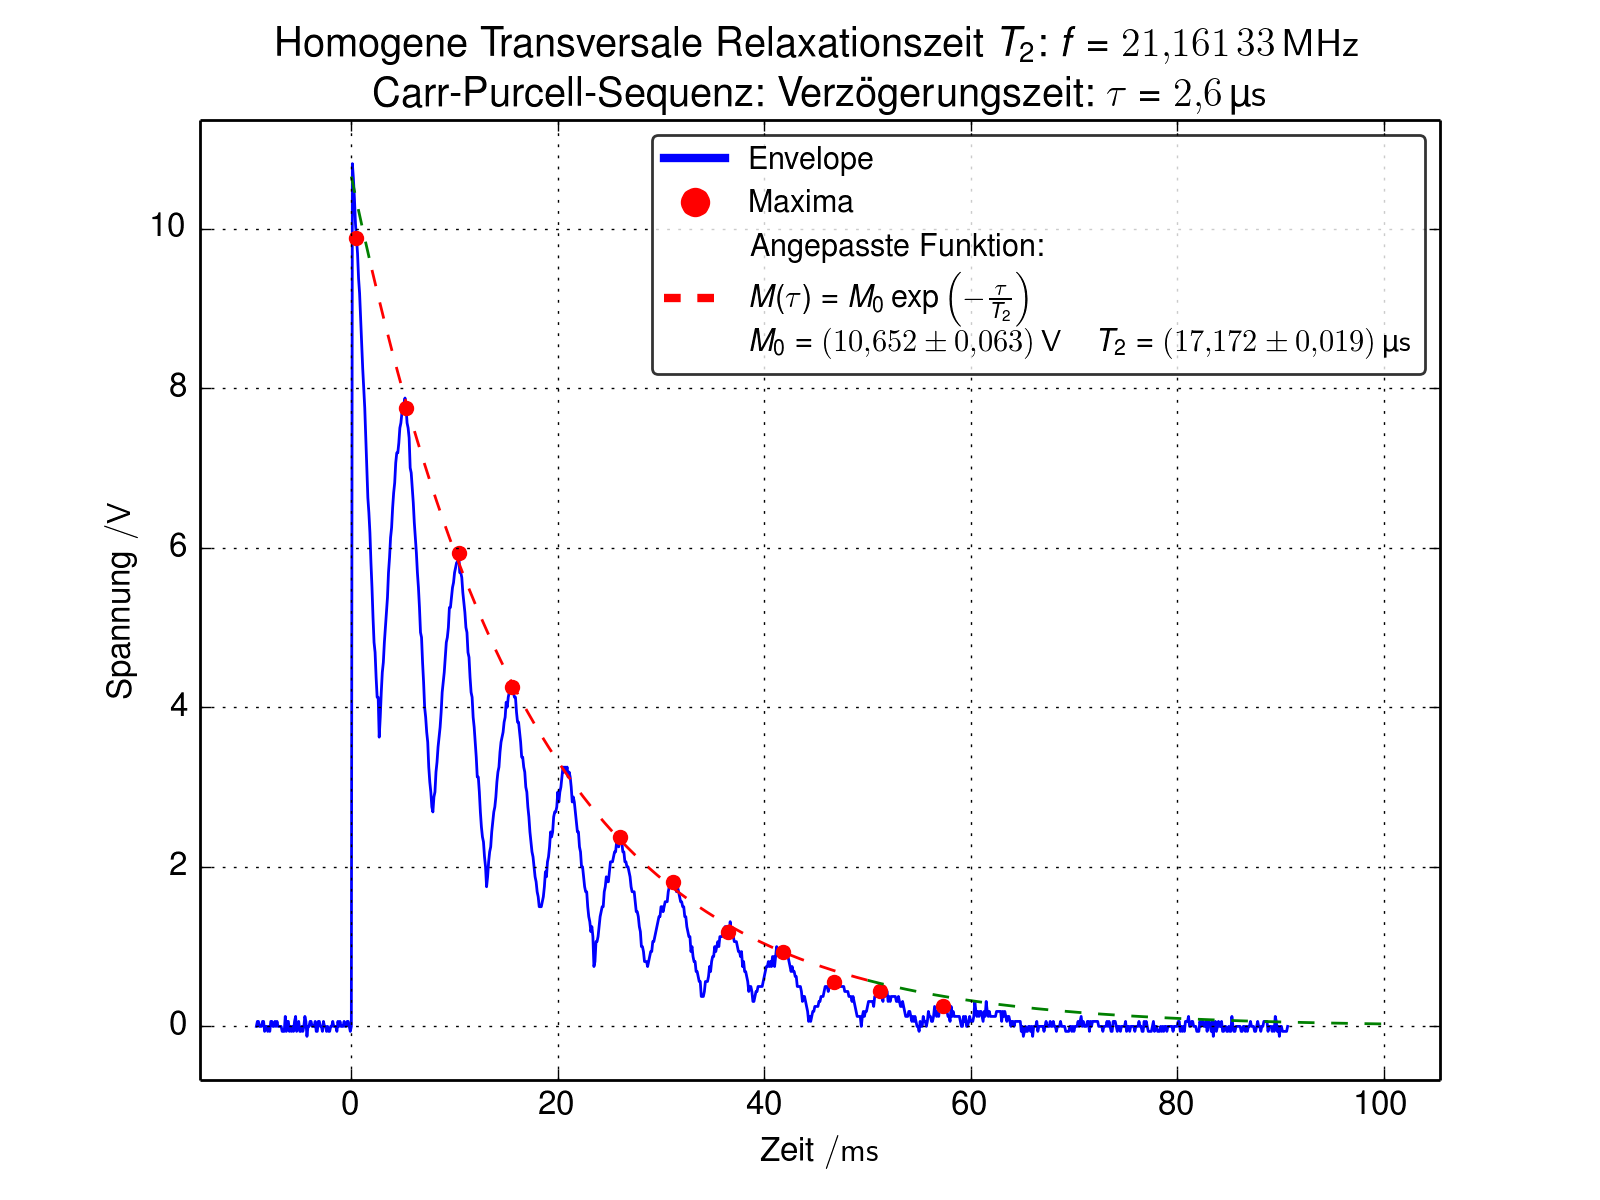
\includegraphics[width=\textwidth]
            {Figures/HomoTransRelax_Carr2.png}
            \caption{Verzögerungszeit von
              $\tau = \SI{2.6}{\micro\second}$.}
            \label{AnhangfigCarr2}
          \end{minipage}\\
          \begin{minipage}{.48\textwidth}
            \centering
            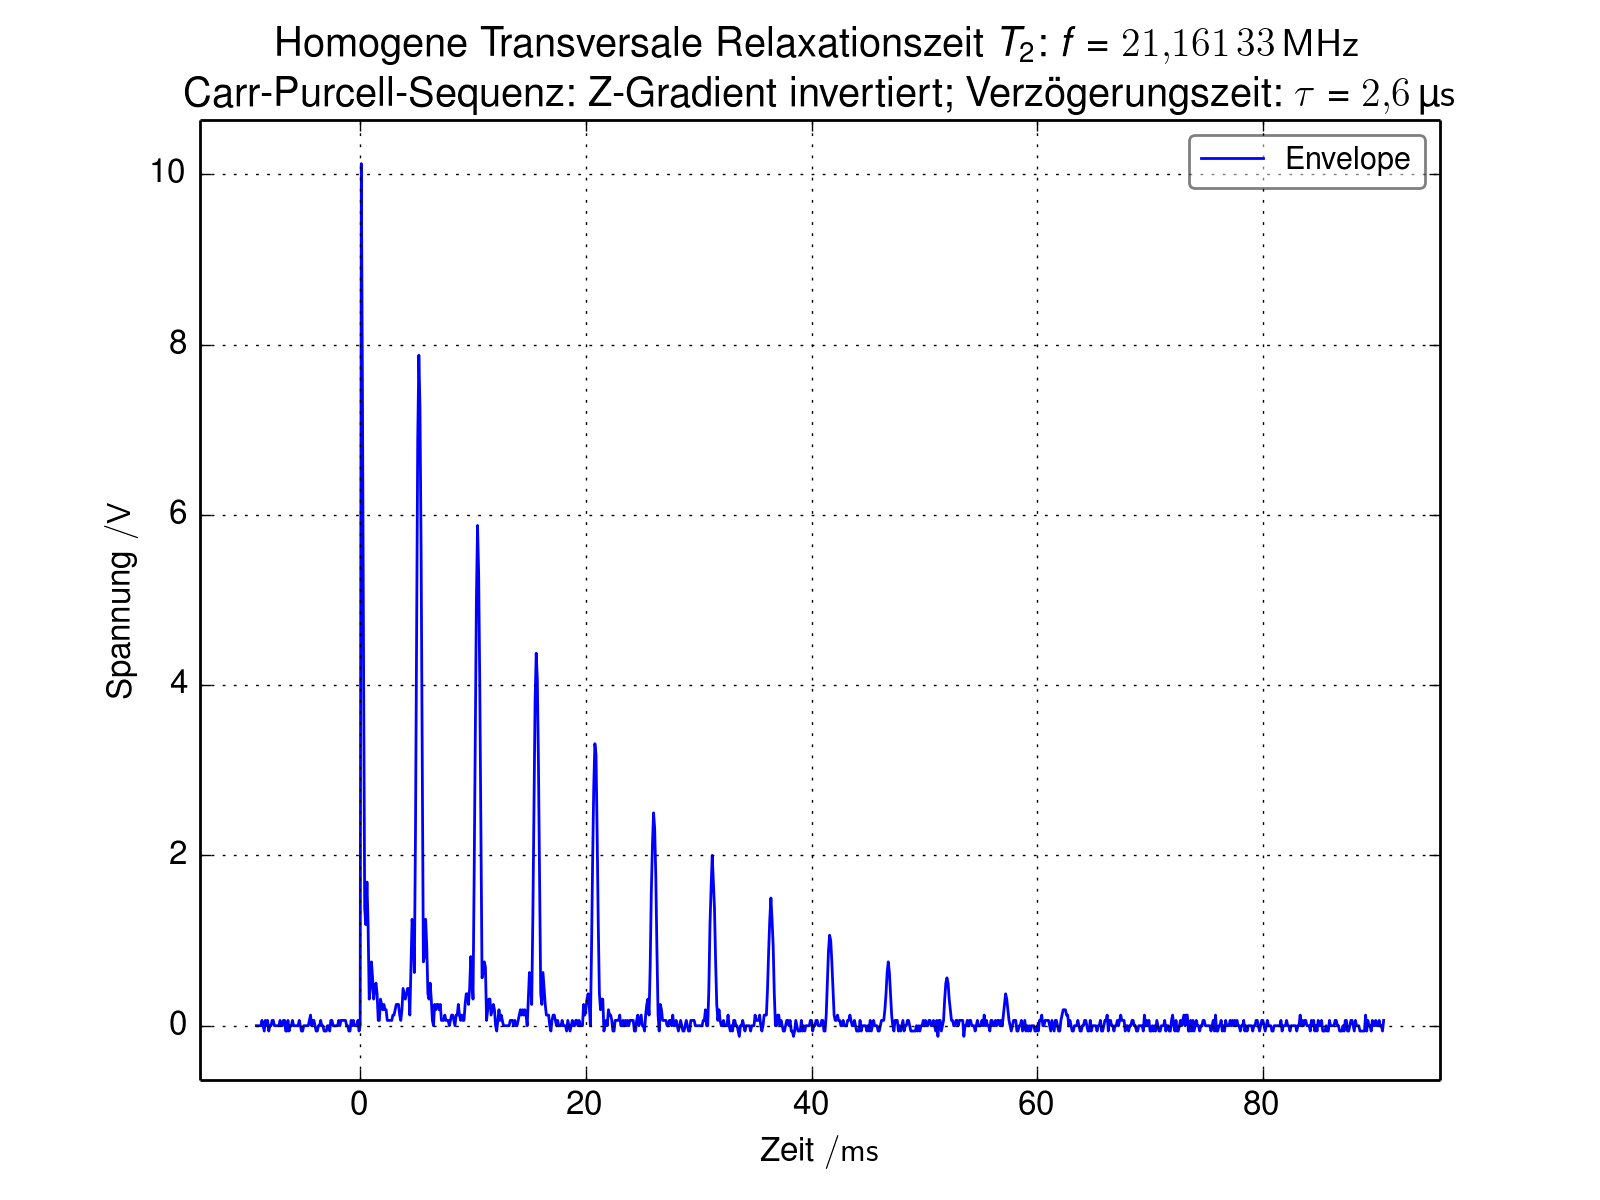
\includegraphics[width=\textwidth]
            {Figures/HomoTransRelax_Carr3.png}
            \caption{Verzögerungszeit von
              $\tau = \SI{2.6}{\micro\second}$ und umgepolten Z-Gradienten.}
            \label{AnhangfigCarr3}
          \end{minipage}\quad
          \begin{minipage}{.48\textwidth}
            \centering
            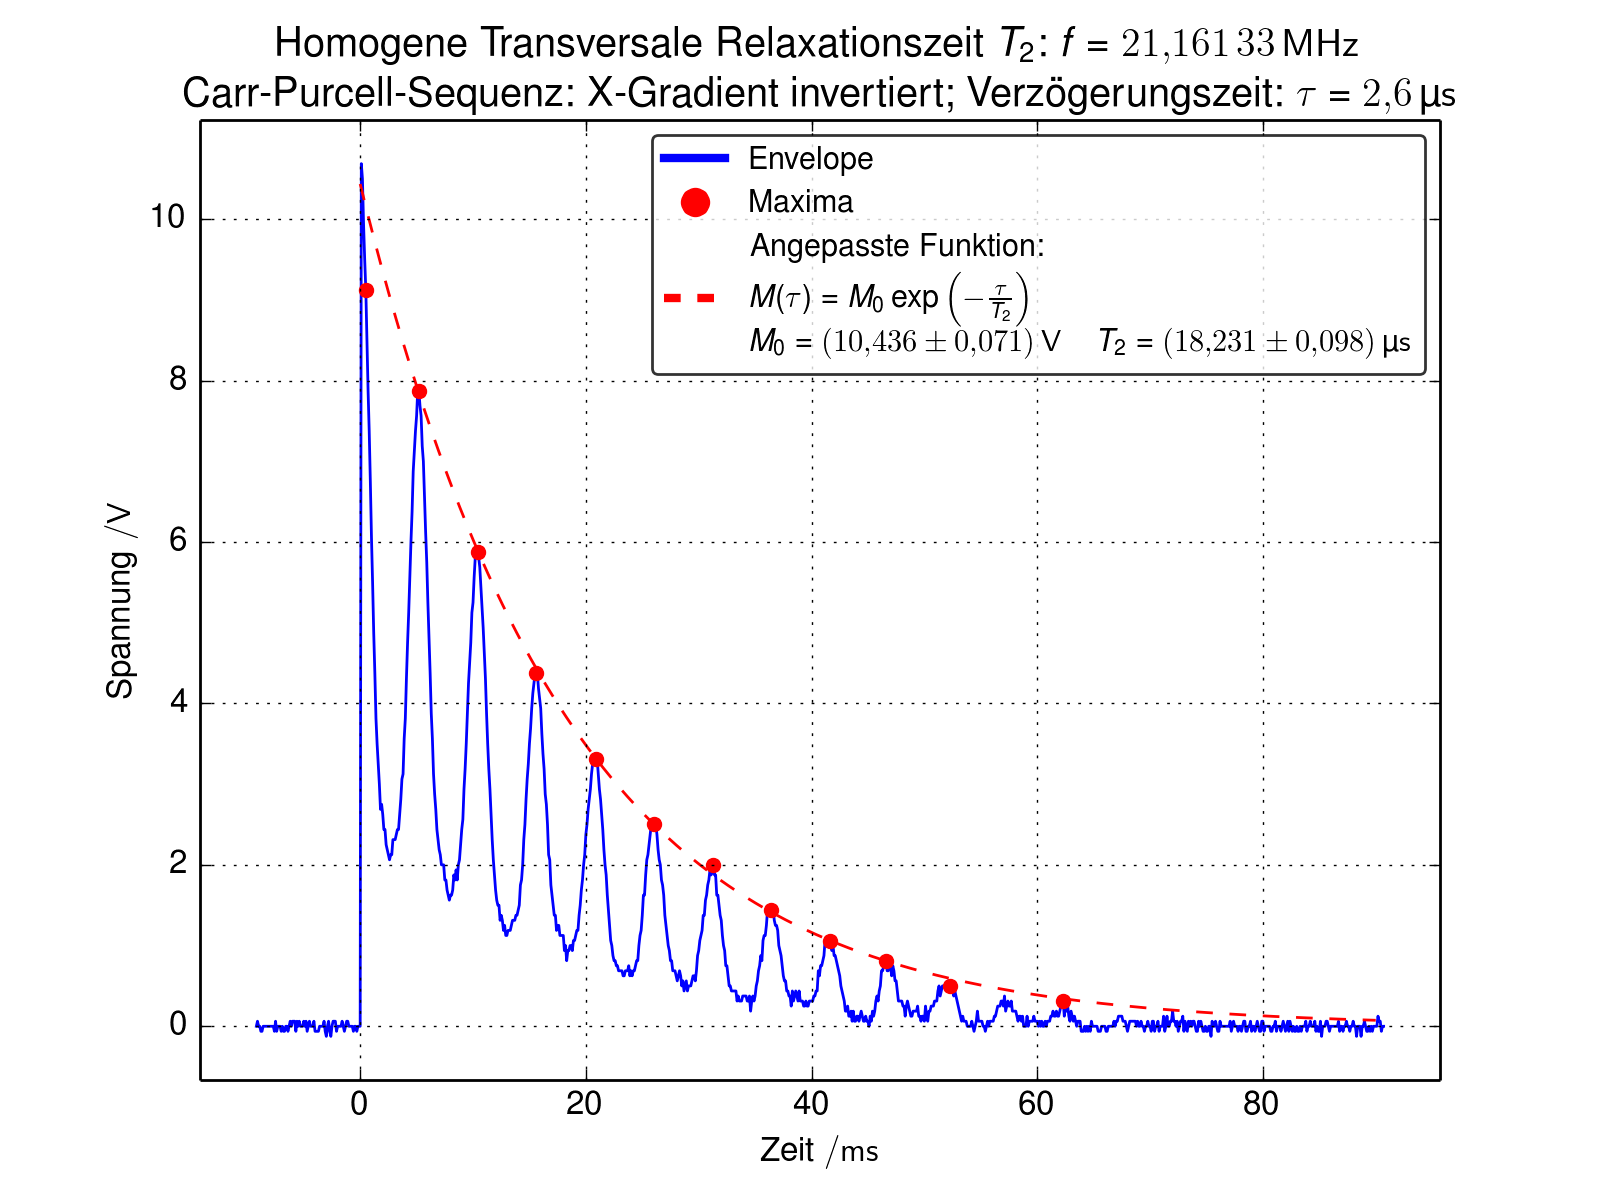
\includegraphics[width=\textwidth]
            {Figures/HomoTransRelax_Carr4.png}
            \caption{Verzögerungszeit von
              $\tau = \SI{2.6}{\micro\second}$ und umgepolten X-Gradienten.}
            \label{AnhangfigCarr4}
          \end{minipage}
          \caption{Verlauf der lokalen Maxima des Antwort - Signales für die
            Carr--Purcell - Sequenz.}
        \end{figure}
        
      \end{subsection}
      %%%%%%%%%%%%%%%%%%%%%%%%%%%%%%%%%%%%%%%
      
      \newpage
      %%%%%%%%%%%%%%%%%%%%%%%%%%%%%%%%%%%%%%%
      %%%%%%%%%%%%%%%%%%%%%%%%%%%%%%%%%%%%%%%
      %%%%%%%%%%%%%%%%%%%%%%%%%%%%%%%%%%%%%%%
      \begin{subsection}*{Meiboom--Gill - Sequenz}
        \label{chpAnhangTransMG}
        \begin{figure}[htb!]
          \centering
          \begin{minipage}{.48\textwidth}
            \centering
            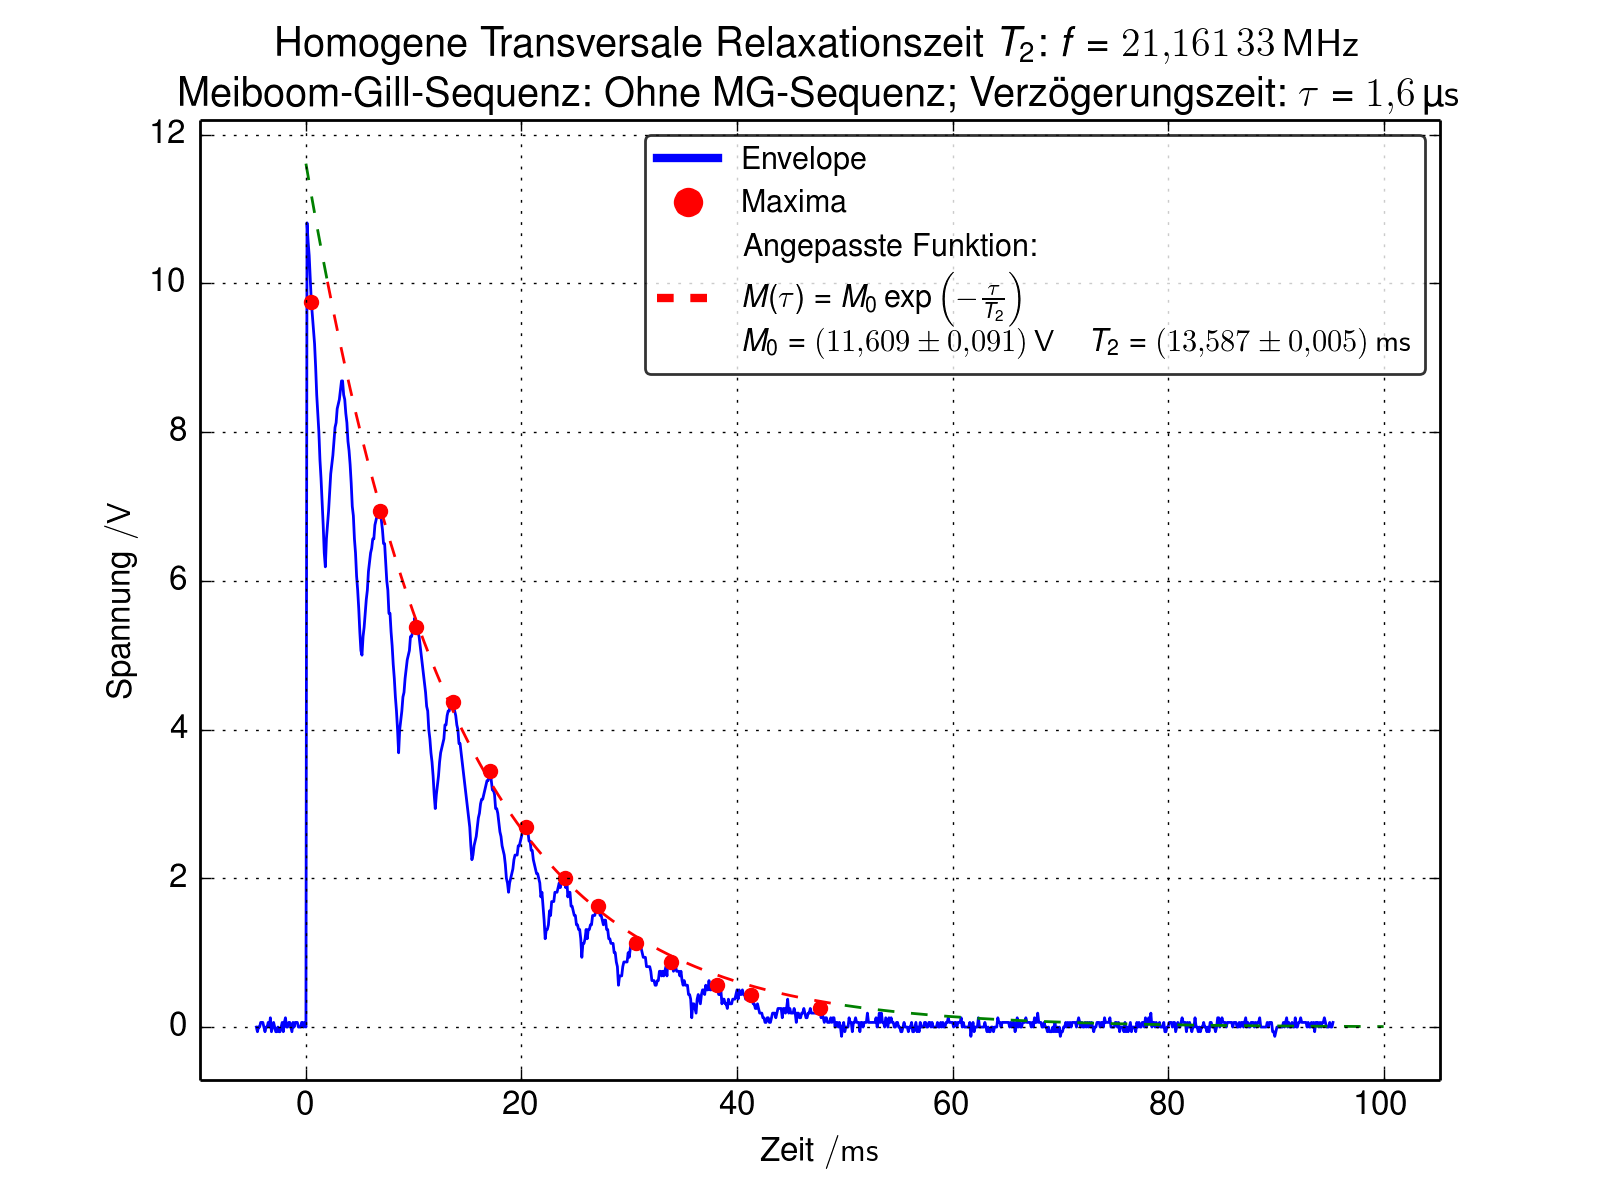
\includegraphics[width=\textwidth]
            {Figures/HomoTransRelax_MG_env0.png}
            \caption{Verlauf der lokalen Maxima des Antwort - Signales für die
              Carr--Purcell - Sequenz bei einer Verzögerungszeit von
              $\tau = \SI{1.6}{\micro\second}$.}
            \label{AnhangfigMG_env0}
          \end{minipage}\quad
          \begin{minipage}{.48\textwidth}
            \centering
            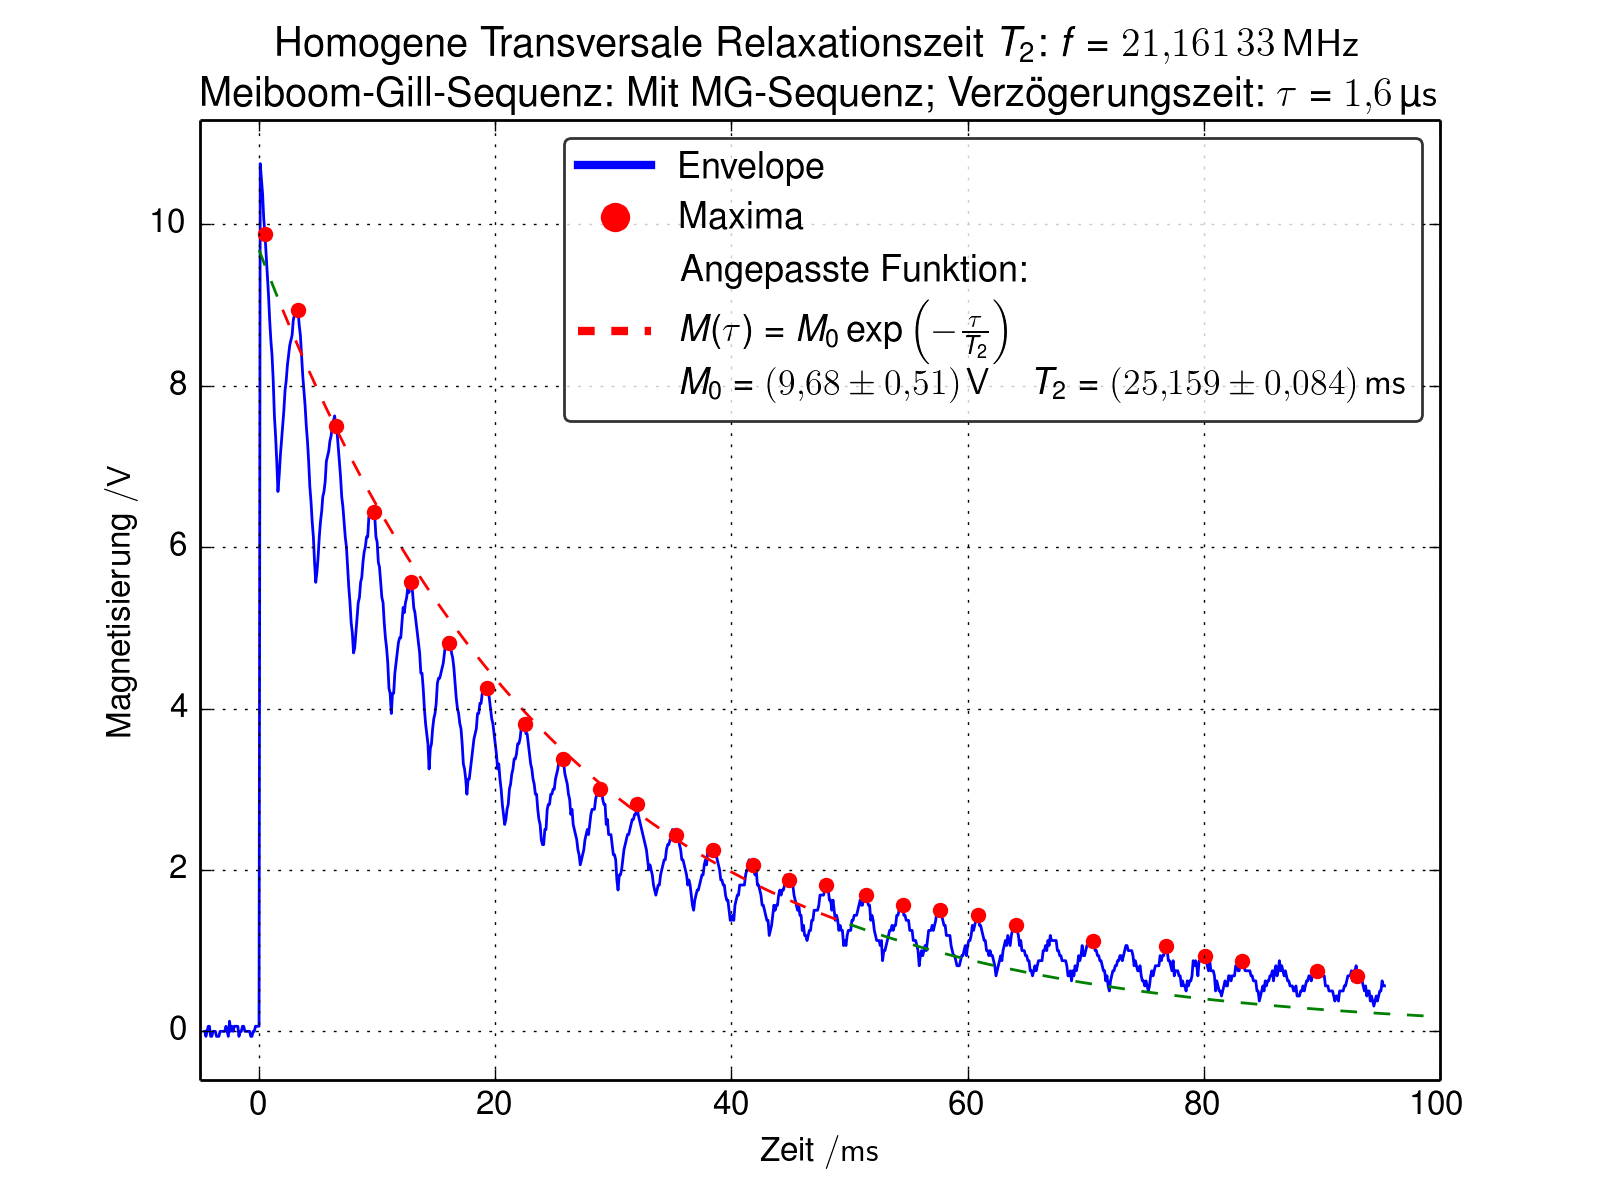
\includegraphics[width=\textwidth]
            {Figures/HomoTransRelax_MG_env1.png}
            \caption{Verlauf der lokalen Maxima des Antwort - Signales für die
              Meiboom--Gill - Sequenz bei einer Verzögerungszeit von
              $\tau = \SI{1.6}{\micro\second}$.}
            \label{AnhangfigMG_env1}
          \end{minipage}
        \end{figure}
        \begin{figure}[htb!]
          \begin{minipage}{.48\textwidth}
            \centering
            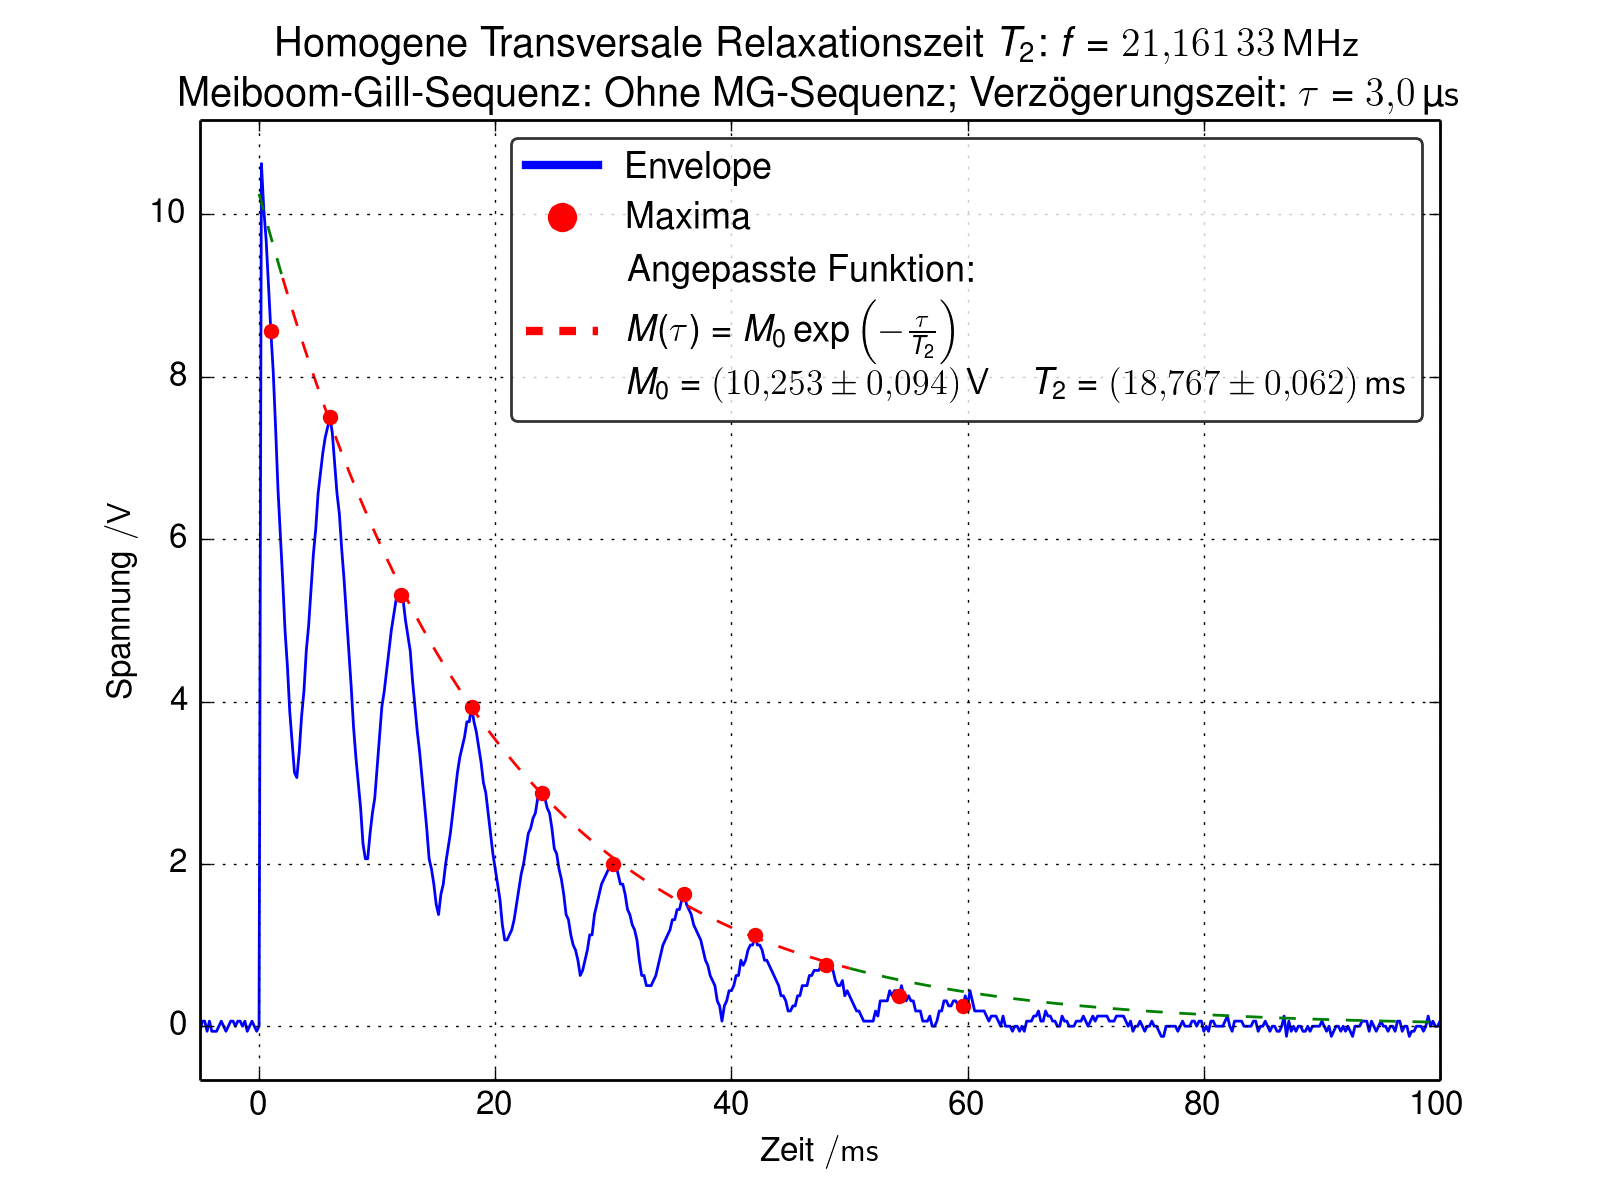
\includegraphics[width=\textwidth]
            {Figures/HomoTransRelax_MG_env2.png}
            \caption{Verlauf der lokalen Maxima des Antwort - Signales für die
              Carr--Purcell - Sequenz bei einer Verzögerungszeit von
              $\tau = \SI{3.0}{\micro\second}$.}
            \label{AnhangfigMG_env2}
          \end{minipage}\quad
          \begin{minipage}{.48\textwidth}
            \centering
            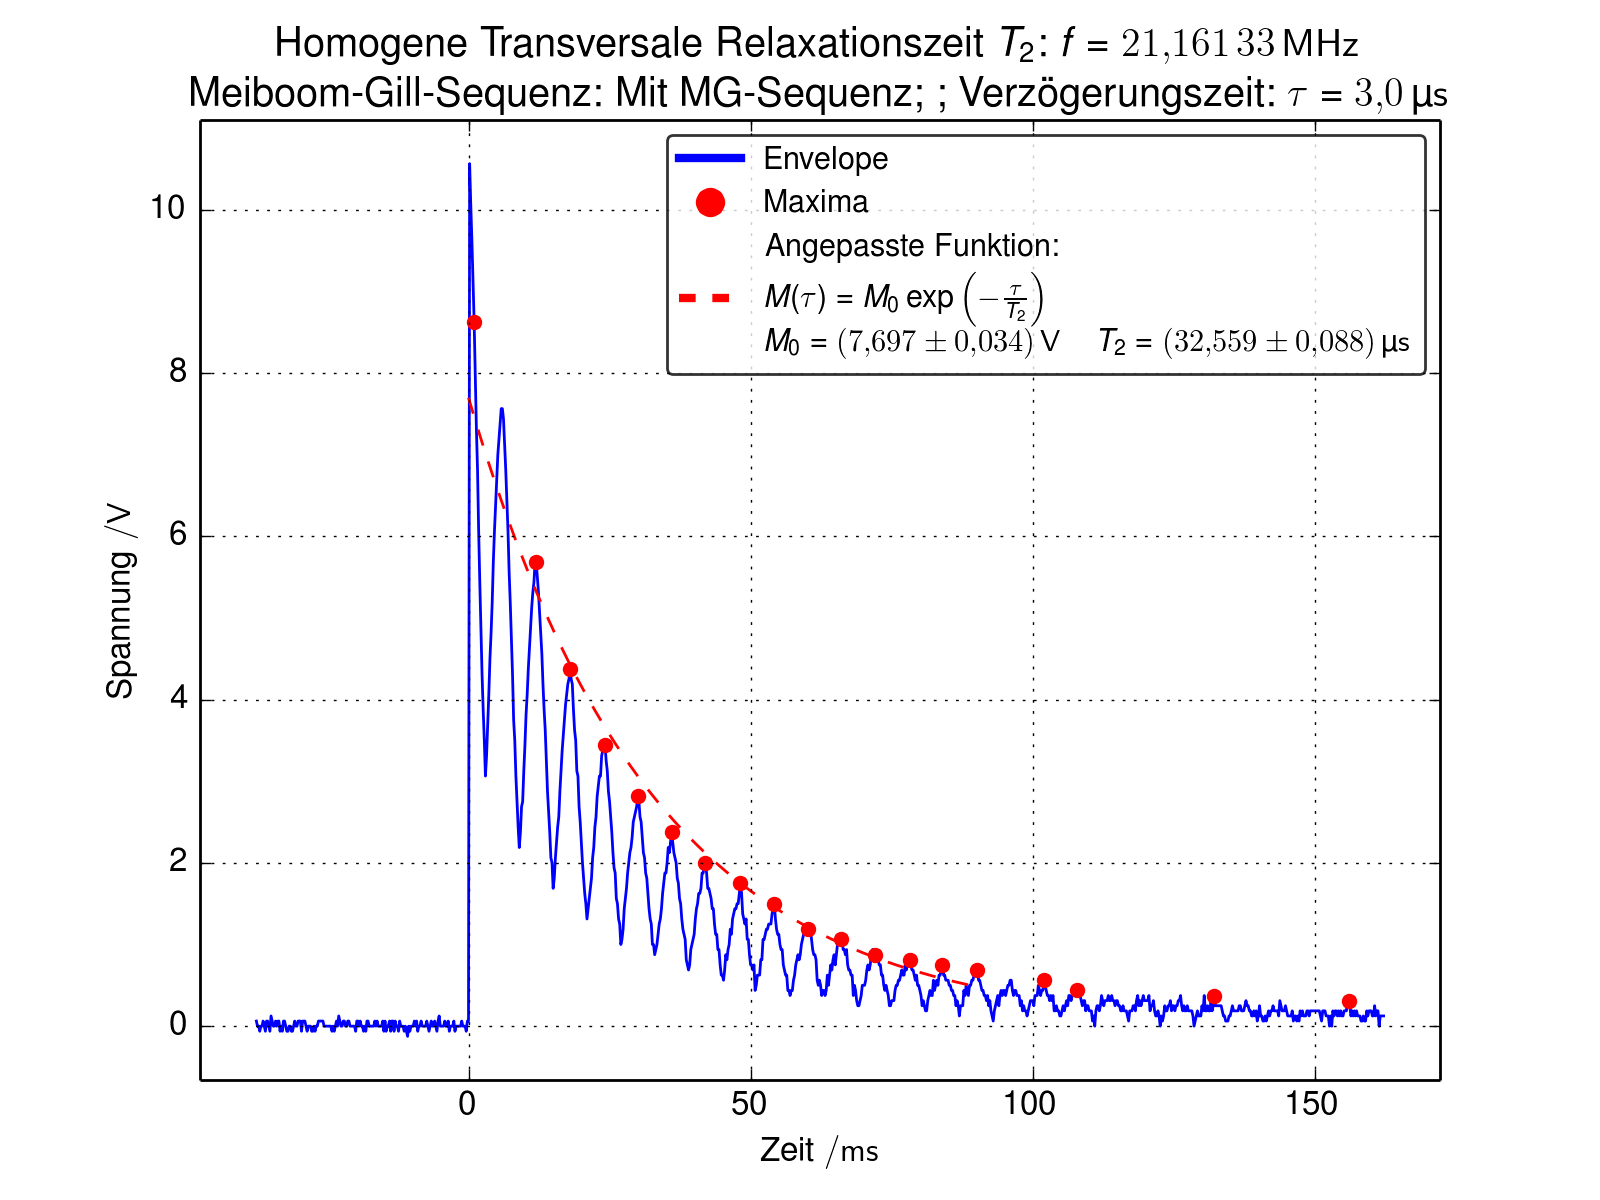
\includegraphics[width=\textwidth]
            {Figures/HomoTransRelax_MG_env3.png}
            \caption{Verlauf der lokalen Maxima des Antwort - Signales für die
              Meiboom--Gill - Sequenz bei einer Verzögerungszeit von
              $\tau = \SI{3.0}{\micro\second}$.}
            \label{AnhangfigMG_env3}
          \end{minipage}
        \end{figure}
        \newpage
        \begin{figure}[htb!]
          \centering
          \begin{minipage}{.48\textwidth}
            \centering
            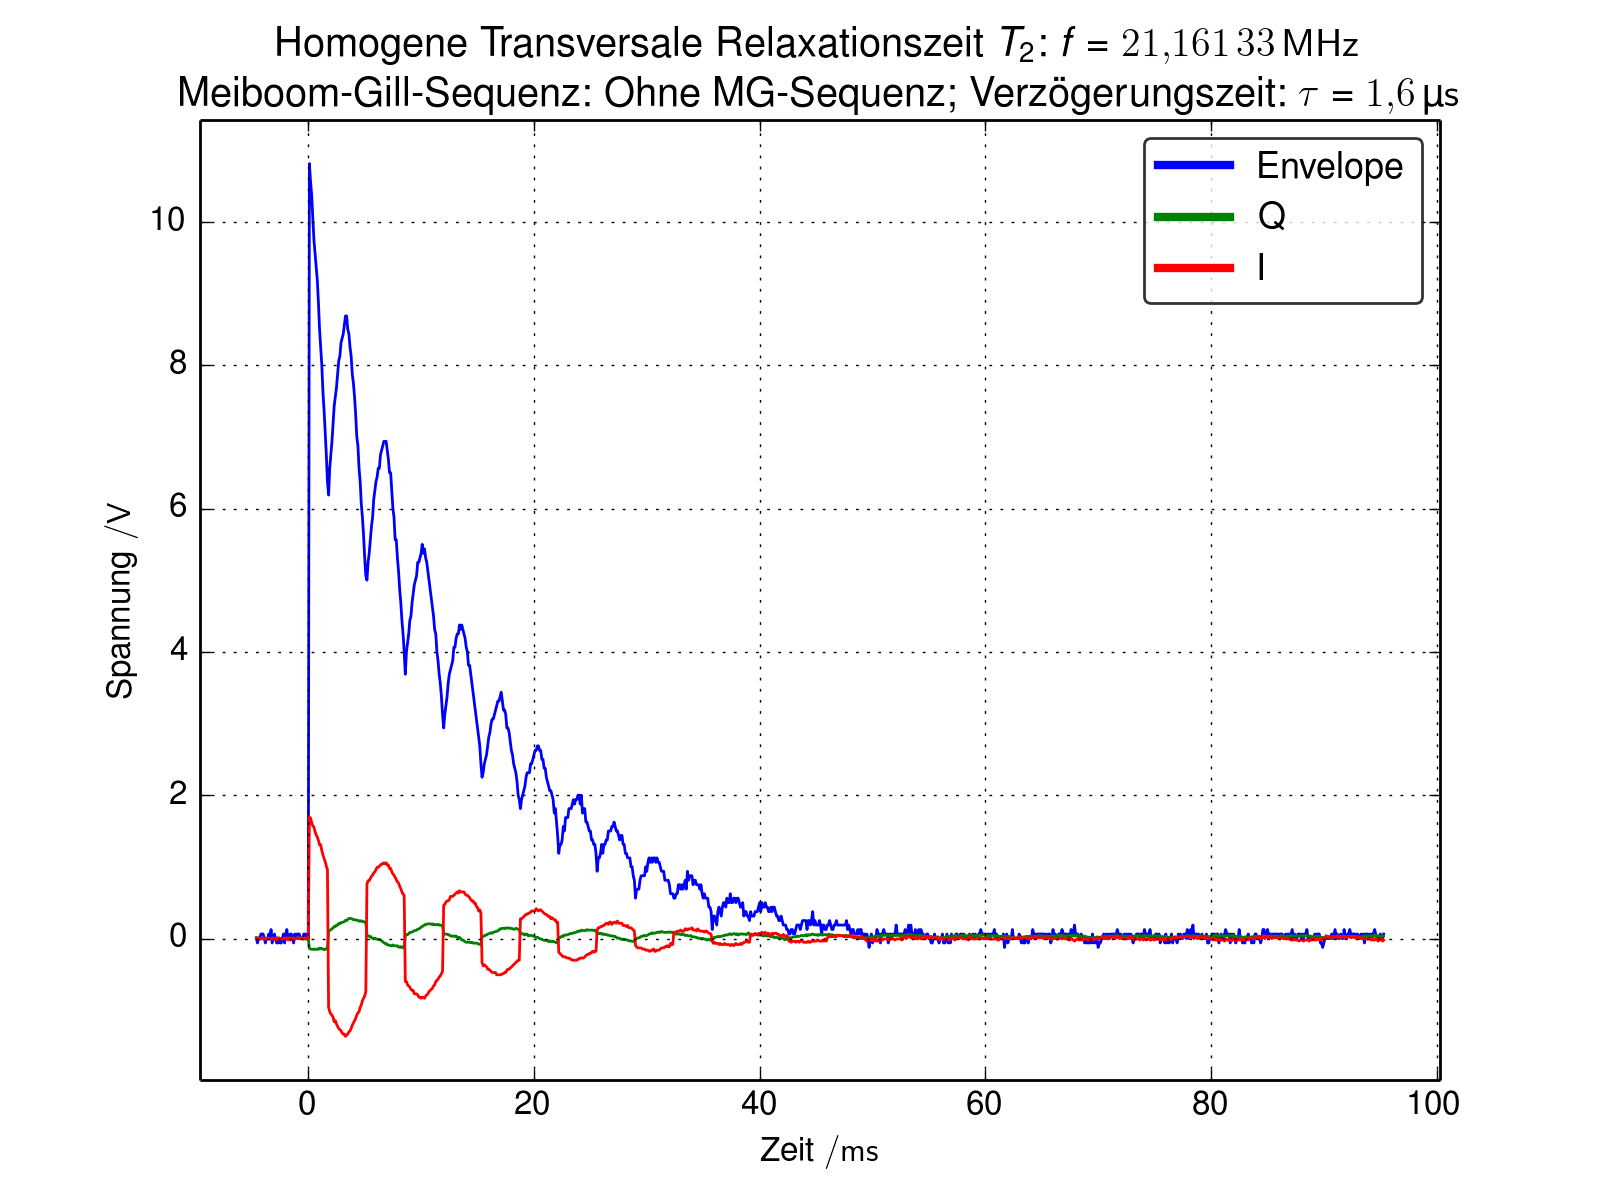
\includegraphics[width=\textwidth]
            {Figures/HomoTransRelax_MG_env_Q_I0.png}
            \caption{Verlauf der Spannungen des Antwort-, Q- und
              In--Phase - Signales bei der Carr--Purcell - Sequenz
              bei einer Verzögerungszeit von $\tau = \SI{1.6}{\micro\second}$.}
            \label{AnhangfigMG_envQI0}
          \end{minipage}\quad
          \begin{minipage}{.48\textwidth}
            \centering
            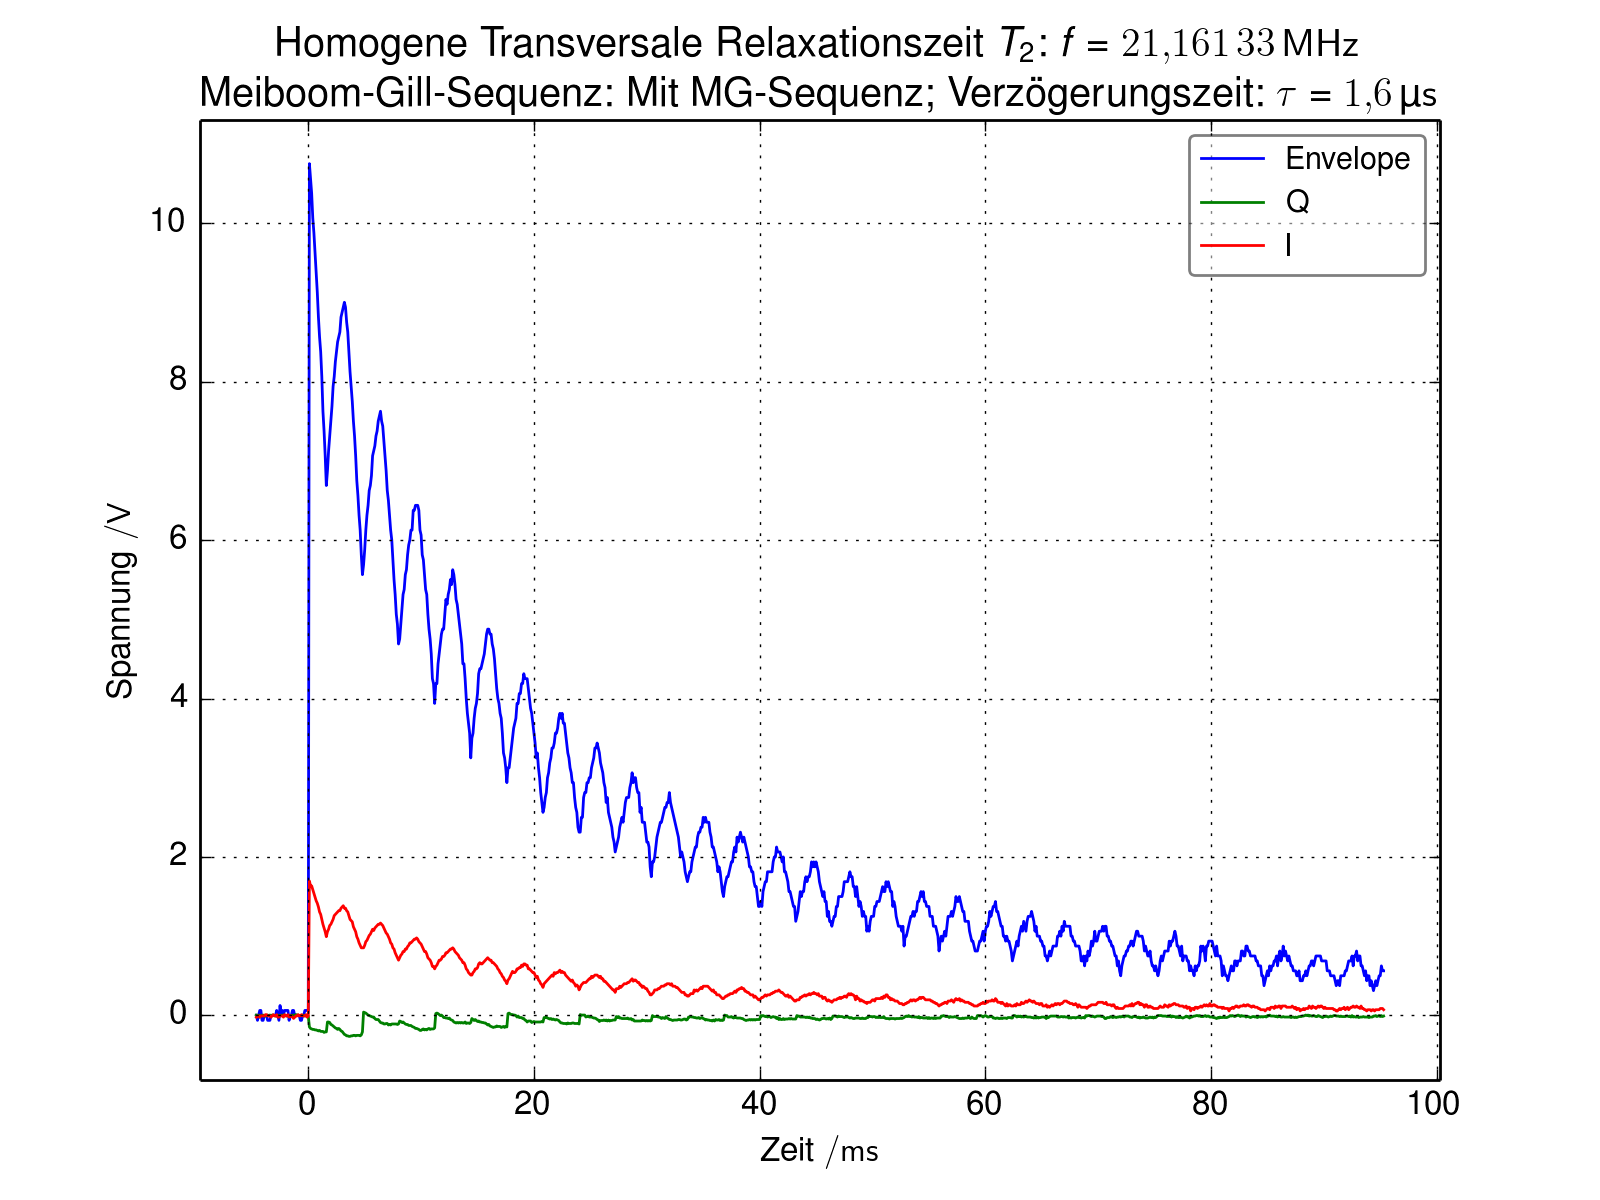
\includegraphics[width=\textwidth]
            {Figures/HomoTransRelax_MG_env_Q_I1.png}
            \caption{Verlauf der Spannungen des Antwort-, Q- und
              In--Phase - Signales bei der Meiboom--Gill - Sequenz
              bei einer Verzögerungszeit von $\tau = \SI{1.6}{\micro\second}$.}
            \label{AnhangfigMG_envQI1}
          \end{minipage}
        \end{figure}
        \begin{figure}[htb!]
          \begin{minipage}{.48\textwidth}
            \centering
            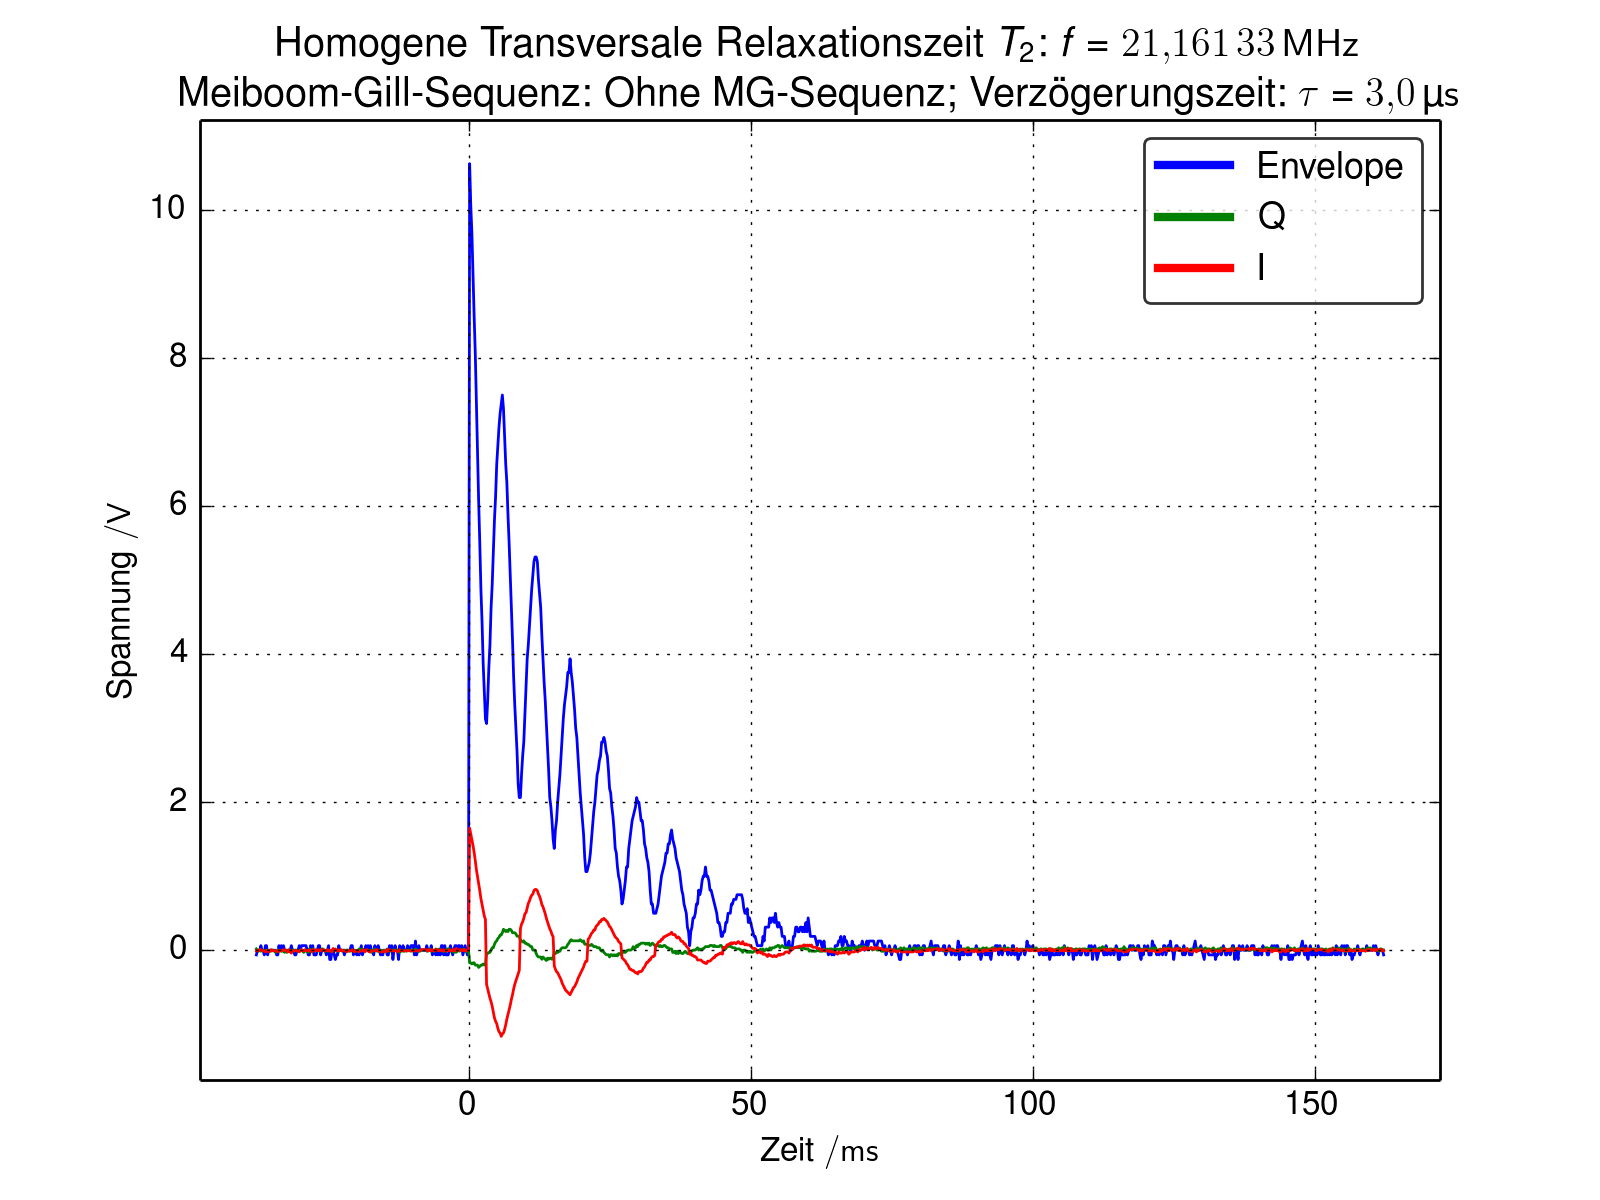
\includegraphics[width=\textwidth]
            {Figures/HomoTransRelax_MG_env_Q_I2.png}
            \caption{Verlauf der Spannungen des Antwort-, Q- und
              In--Phase - Signales bei der Carr--Purcell - Sequenz
              bei einer Verzögerungszeit von $\tau = \SI{3.0}{\micro\second}$.}
            \label{AnhangfigMG_envQI2}
          \end{minipage}\quad
          \begin{minipage}{.48\textwidth}
            \centering
            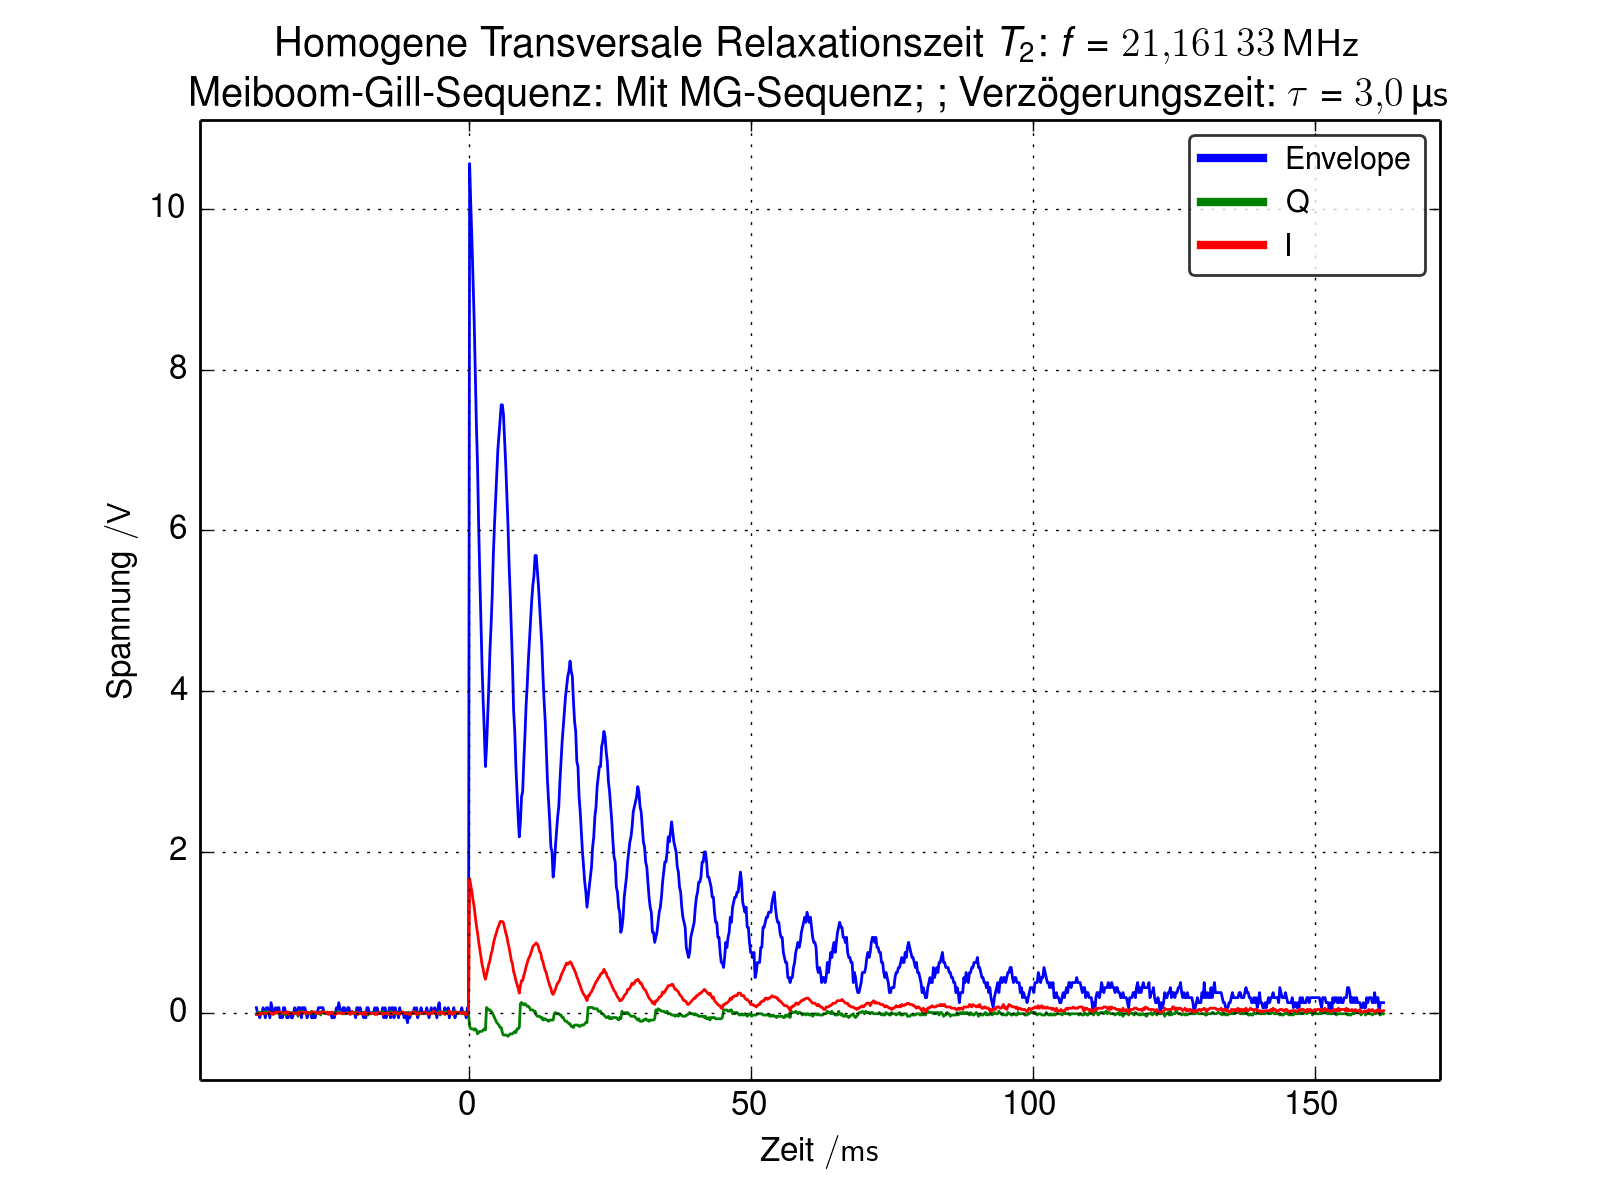
\includegraphics[width=\textwidth]
            {Figures/HomoTransRelax_MG_env_Q_I3.png}
            \caption{Verlauf der Spannungen des Antwort-, Q- und
              In--Phase - Signales bei der Meiboom--Gill - Sequenz
              bei einer Verzögerungszeit von $\tau = \SI{3.0}{\micro\second}$.}
            \label{AnhangfigMG_envQI3}
          \end{minipage}
        \end{figure}
        
      \end{subsection}
      %%%%%%%%%%%%%%%%%%%%%%%%%%%%%%%%%%%%%%%
      
    \end{section}
    %%%%%%%%%%%%%%%%%%%%%%%%%%%%%
    
  \end{chapter}
  %%%%%%%%%%%%%%%%%%%%%%%%%%%%%%
  
\end{appendix}
%%%%%%%%%%%%%%%%%%%%
 